% Created 2016-05-16 Mon 02:22

\documentclass[14pt, a4paper]{extreport}

\newcommand{\comment}[1]{}

\usepackage{hyperref}
\usepackage{graphicx}
\usepackage[utf8]{inputenc}
\usepackage[T1, T2A]{fontenc}
\usepackage{fixltx2e}
\usepackage{grffile}
\usepackage{longtable}
\usepackage{wrapfig}
\usepackage{rotating}
\usepackage[normalem]{ulem}
\usepackage{amsmath}
\usepackage{textcomp}
\usepackage{amssymb}
\usepackage{capt-of}
\usepackage{listings}
\usepackage{totcount}
\usepackage[figure,table]{totalcount}
\usepackage{etoolbox}
\usepackage{tocvsec2}
\usepackage{booktabs}

\setcounter{secnumdepth}{2}

\regtotcounter{page}

\newtotcounter{citenum}
\def\oldcite{}
\let\oldcite=\bibcite
\def\bibcite{\stepcounter{citenum}\oldcite}

\newtotcounter{attachcnt}

\usepackage{indentfirst}
\usepackage[left=3cm,right=1cm,
  top=2cm,bottom=2cm,bindingoffset=0cm]{geometry}
\usepackage[nodisplayskipstretch]{setspace}
\onehalfspacing
\sloppy
%\parindent=1cm

\usepackage{enumitem}
\setlist{nolistsep}

\usepackage{titlesec}

\usepackage{etoolbox}

\makeatletter
\patchcmd{\ttlh@hang}{\parindent\z@}{\parindent\z@\leavevmode}{}{}
\patchcmd{\ttlh@hang}{\noindent}{}{}{}
\makeatother


\titleformat{\chapter}[display]{\filcenter\bfseries\Large}{}{8pt}{}{}
\titleformat{\section}{\bfseries\Large}{\thesection}{1em}{}{}
\titleformat{\subsection}{\bfseries\normalsize}{\thesubsection}{1em}{}{}
\titleformat{\subsubsection}{\bfseries\normalsize}{\thesubsubsection}{1em}{}{}

% Настройка вертикальных и горизонтальных отступов
\titlespacing*{\chapter}{0pt}{-30pt}{*2}
\titlespacing*{\section}{\parindent}{*2}{*1}
\titlespacing*{\subsection}{\parindent}{*2}{*1}
\titlespacing*{\subsubsection}{\parindent}{*0.5}{*0}

\usepackage{polyglossia}
\setdefaultlanguage[spelling=modern]{russian}
\setotherlanguage{english}
\defaultfontfeatures{Mapping=tex-text}
\newfontfamily{\cyrillicfont}{Times New Roman}
\newfontfamily{\cyrillicfonttt}{Courier New} % шрифт URL-ссылок
%\newfontfamily{\sourcecodefont}{Courier New}
\defaultfontfeatures{Ligatures={TeX},Renderer=Basic}    %% свойства шрифтов по умолчанию
\setmainfont[Ligatures={TeX,Historic}]{Times New Roman} %% задаёт основной шрифт документа
%% \setsansfont{CMU Sans Serif}                         %% задаёт шрифт без засечек
\setmonofont{Courier New}                               %% задаёт моноширинный шрифт

\newcommand{\fixedspaceword}[2][1]{%
  \begingroup
  \spaceskip=#1\fontdimen2\font
  \xspaceskip=0pt\relax % just to be sure
  #2%
  \endgroup
}

% объявляем новую команду для переноса строки внутри ячейки таблицы
\newcommand{\spcell}[2][c]{%
  \begin{tabular}[#1]{@{}c@{}}#2\end{tabular}}

\bibliographystyle{gost705}

\makeatletter
\def\@biblabel#1{#1. }
\makeatother

\usepackage{caption}
\AtBeginDocument{%
  \def\contentsname{ОГЛАВЛЕНИЕ}
  \def\bibname{СПИСОК ИСПОЛЬЗОВАННОЙ ЛИТЕРАТУРЫ}
  \renewcommand{\figurename}{Рисунок}
  \renewcommand{\tablename}{Таблица}
  \renewcommand{\thefigure}{\arabic{chapter}.\arabic{figure}}
  \renewcommand{\thetable}{\arabic{chapter}.\arabic{table}}
  \renewcommand{\theequation}{\arabic{chapter}.\arabic{equation}}
}

\author{Великий Студент Анонимович}
\date{\today}

\title{Дипломная работа\\
  <<Методы написания дипломной работы в последний момент перед предзащитой>>}

\hypersetup{
  pdfauthor={Великий С.А.},
  pdftitle={Методы написания дипломной работы в последний момент перед предзащитой},
  pdfkeywords={СПИСОК КЛЮЧЕВЫХ СЛОВ, КАСАЮЩИХСЯ ТЕМЫ РАБОТЫ},
  pdfsubject={Тема работы},
  pdfcreator={xelatex},
  pdflang={Russian}}


\begin{document}

%%% начало документа
%%% заглушка титульного листа, настоящий делать на основе образца в файле Titul.doc

\maketitle

%%% описание рефератов

\setcounter{page}{2}

\settocdepth{chapter}

\chapter*{РЕФЕРАТ}
Дипломная работа: \total{page}\ страниц, \totalfigures{}~иллюстраций, \totaltables{}\ таблиц,
\total{citenum}\ источников, \total{attachcnt}\ приложений.

\vspace{\baselineskip}

СПИСОК КЛЮЧЕВЫХ СЛОВ ЗАГЛАВНЫМИ БУКВАМИ, ЧЕРЕЗ ЗАПЯТУЮ

\vspace{\baselineskip}

Текст реферата.


\chapter*{РЭФЕРАТ}
Дыпломная праца: \total{page}\ старонак, \totalfigures{}~iллюстрацый, \totaltables{}~таблiц,
\total{citenum}\ крынiц, \total{attachcnt}\ дадаткаў.

% ў Ў

\vspace{\baselineskip}

СПИСОК КЛЮЧЕВЫХ СЛОВ ЗАГЛАВНЫМИ БУКВАМИ, ЧЕРЕЗ ЗАПЯТУЮ, НА БЕЛОРУССКОМ ЯЗЫКЕ

\vspace{\baselineskip}

Текст реферата на белорусском языке.


\chapter*{ABSTRACT}
Graduate thesis: \total{page}\ pages, \totalfigures{}~figures, \totaltables{}\ tables,
18 citations, 1 attachment.

\vspace{\baselineskip}

EXON, DATA PROCESSING, HIERARCHICAL CLUSTERING, SPECTRAL CLUSTERING, FEATURE IMPORTANCE RANKING, DIMENSIONALITY REDUCTION, CLUSTERING EVALUATION

\vspace{\baselineskip}

The object of research is the development of algorithm for automatic ranking and selection of most important features of the oncogene exon.

The goal of study is to develop and study algorithms for automatic selection of the most important features of exons and algorithms for cluster analysis of oncogene exons.

The approaches for determining the importance of features in clustering is investigated, the algorithms of initial data clustering are studied and selected, the simulation model of data generation is developed, the algorithm for determining the importance of features is developed on the basis of studied approaches, the influence of data preprocessing on the ranking of features is investigated, the method for estimating and evaluating of feature importance score is developed.

As a result of the work, the algorithm was developed for selecting the most important features of the oncogene exon, including preprocessing of data, a procedure for ranking and selecting features, and constructing an interpreted selection result. Discussion and analysis of the data were carried out, the algorithm was evaluated.


%%% оглавление

\tableofcontents

%%% описание введения

\phantomsection
\chapter*{ВВЕДЕНИЕ}
\addcontentsline{toc}{chapter}{Введение}

Lorem ipsum dolor sit amet, consectetur adipiscing elit. Fusce ultrices finibus arcu in tincidunt.
Curabitur pellentesque purus vel aliquet efficitur. Morbi quis placerat diam. Curabitur id fringilla
nibh, eu volutpat tellus. Sed nec fermentum magna, eget blandit ipsum. Aenean fermentum ipsum eu
luctus vulputate. In hendrerit eros nibh, non pretium eros malesuada nec. Donec enim lectus, convallis
id scelerisque a, molestie nec neque.

Integer fermentum, dui volutpat suscipit scelerisque, orci sapien suscipit mauris, nec bibendum est
enim elementum sem. Mauris pharetra turpis eget ex tincidunt, in efficitur mi dictum. Suspendisse
convallis non lacus nec fermentum. Suspendisse eleifend enim odio, sed eleifend felis luctus eget.
In bibendum nulla a lorem tempor dignissim. Nunc tempor arcu a nisl feugiat, a fermentum ante eleifend.
Etiam sed augue lacinia, luctus odio sed, dapibus lacus. Pellentesque suscipit mauris vitae est
fringilla consequat. Sed dui est, varius sit amet auctor ut, euismod a magna. Vivamus tristique leo
ligula, non lacinia justo volutpat in. Maecenas eu mi velit. Sed vel elit ligula. In imperdiet varius
elit, at rutrum mauris lobortis nec. Suspendisse quis orci id urna porta eleifend.

Curabitur pellentesque nunc ut urna elementum bibendum. Maecenas sit amet ante tincidunt, dictum
neque et, eleifend felis. Pellentesque rhoncus mi ut mauris ullamcorper pretium. Maecenas non blandit
ex, quis elementum leo. Donec ultricies, velit in ultricies fringilla, turpis neque facilisis eros,
non congue ipsum sapien id enim. Praesent vitae tellus ornare orci mattis ornare et ut sapien. Quisque
iaculis lorem mauris. Phasellus eu arcu placerat, convallis velit at, tincidunt velit. Nulla eget
vestibulum erat. Fusce eu ipsum rutrum, varius felis dictum, aliquam augue.

In dignissim odio eget porttitor malesuada. Pellentesque venenatis urna eget risus facilisis
imperdiet. Donec ligula neque, volutpat ut leo in, interdum pellentesque metus. Nam mattis ligula
nec volutpat fringilla. Pellentesque nec semper mauris, non condimentum metus. Ut imperdiet sapien
nec pretium porta. Nam id arcu non nibh ultricies consectetur id sed dui.

Duis semper luctus posuere. Donec aliquet quam a ex posuere venenatis. Aliquam interdum suscipit
justo, placerat auctor lacus feugiat eget. Aliquam vulputate vitae lorem at molestie. In iaculis
felis in felis rutrum, eget finibus nunc gravida. Curabitur tortor tortor, rutrum eu urna ut, commodo
tempor justo. Quisque at tortor nec leo fringilla posuere.

Fusce sapien nisl, gravida et eleifend vitae, finibus at quam. Curabitur quis venenatis nisl.
Aenean in rhoncus magna. In hac habitasse platea dictumst. Nulla id feugiat nibh. Suspendisse ut
ligula at elit auctor aliquet. Quisque dolor nunc, pretium vitae posuere dapibus, molestie ac lectus.
Nulla tempor dui lacinia auctor finibus. Curabitur placerat diam non augue posuere accumsan. Nunc
laoreet urna mi, eget faucibus ligula faucibus at. Nunc eu laoreet erat. Suspendisse varius est orci,
ut scelerisque metus faucibus non. Donec luctus et massa non semper. Nullam non augue enim. Aliquam
vitae convallis ligula. Interdum et malesuada fames ac ante ipsum primis in faucibus.

\begin{figure}
  
\includegraphics[width=\linewidth]{pics/hardcore.jpg}
  \caption{Учеба - это хардкор. Диплом - это дважды хардкор.}
  %\label{fig:hard}
\end{figure}



\settocdepth{subsection}

%%% описание главы 1

\stepcounter{chapter}
\phantomsection
\chapter*{ГЛАВА 1\\
  ТЕОРЕТИЧЕСКАЯ ЧАСТЬ}
\addcontentsline{toc}{chapter}{Глава 1. Теоретическая часть}
\setcounter{section}{0}

\thesection[Модель исследования]{Модель исследования}
\subsection{Описание CRISP-DM}
CRISP-DM(CRoss-Industry Standart Process for Data Mining) -- независимый от приложений универсальный процессный стадарт для обработки данных. Как любой процессный стандарт, он имеет иерархическую структуру: фазы, общие задачи, специализированные задачи, отдельные процессы. Целью методологии является представление решения задачи как последовательность дискретных событий, допускающий параллельную обработку, плагирование, делегирование. \cite{azevedo2008kdd}

На верхнем уровне процесс обработки данных организован как набор фаз, сменяющих друг друга, каждая фаза состоит из нескольких общих задач. Задачи называются общими, потому что они формулируются с целью покрытия все возможных ситуаций в анализе данных. Решения общих задач должны быть завершенными и стабильными. Завершенными с точки зрения предоставления результата, удовлетворяющего исходной формулировке и стабильными с точки зрения масштабируемости под следующую фазу и совместимости с её задачами.

Уровень специализированных задач конкретизирует общие задачи применительно к конкретному набору данных. Например общей задаче <<подготовка данных>> могут соответствовать специализированные задачи <<стандартизация>>, <<удаление выбросов>>, <<кодирование категориальных переменных>>.

Четвертый уровень содержит процессы решения каждой конкретной задачи как последовательность решений, действий и результатов. Процесс представляет собой развитие действий в каждой задаче.

\subsection{Контекст анализа данных}
CRISP-DM вводит соответствие общими и специализированными уровнями в анализе данных. Рассматривается четыре аспекта анализа данных:
\begin{itemize}
	\item \textbf{Область приложения}, определяет область знания, откуда идет задача
	\item \textbf{Тип задачи анализа данных}, определяет специфическую цел анализа данных, преследуемую проектом
	\item \textbf{Аспект специфики}, определяет возможные сложные ситуации, возникающие в анализе данных
	\item \textbf{Технический аспект}, определяет техники и инструменты анализа данных, применяемые в данной задаче 
\end{itemize}

Каждый контекст включает в себя один или больше перечисленных аспектов. 

\subsection{Модель CRISP-DM}
Модель CRISP-DM представляет собой жизненный цикл проекта анализа данных и содержит все его фазы, задачи, и отношения между фазами и задачами. Отношения могут существовать между данными, между задачами, могут приходить из области приложения и других источников. \cite{azevedo2008kdd}

Модель состоит из шести фаз. Переходы между фазами происходят не только вперёд, переходы назад или переходы через фазу тоже иногда небходимы. Результат каждой фазы определяет следующую фазу или конкретную задачу. Стрелки обозначают наиболее общие и частые переходы между фазами. Рассмотрим фазы CRISP-DM:
\begin{enumerate}
	\item \textit{Понимание цели приложения}

	Начальная фаза предполагает изучения целей проекта в прилагаемой области и формулирование из предметной задачи задачи анализа данных и разработку плана для её решения.
	\item \textit{Понимание данных}

	Вторая фаза начинается со сбора данных, и включает в себя знакомство с содержанием и качеством данных, детектирование аномалий, построение выборок и построение гипотез.
	\item \textit{Подготовка данных}

	Фаза подготовки данных включает в себя все действия, необходимые для подготовки финального исследуемого набора данных из полученных на второй фазе сырых данных. Задания включают в себя миграцию, очистку, выбор атрибутов, трансформацию данных с использованием специализированных инструментов.
	\item \textit{Моделирование}

	На данной фазе иденцифицируются и решаются задачи анализа данных, подбираются целевые величины для оптимизации, проверяются сделанные гипотезы. Часто требуется возвращение ко второй фазе.
	\item \textit{Валидация}

	Фаза состоит в оценке качества построенной модели с точки зрения метрик анализа данных, производится проверка шагов, сделанных при построении модели, связь метрики анализа данных с целями, поставленными в первой фазе. К концу фазы предполагается использование в области приложения результатов модели.
	\item \textit{Развёртывание}

	Создание модели не означает собой конец проекта. Как только модель способна производить знания, её использование должно быть организовано и задокументировано, для удобства конечного пользователя. Так же модель должна быть гибкой и поддерживаемой. Результатом фазы является готовый программный продукт, пригодный к внедрению.
\end{enumerate}  
\subsection{Основные результаты и выводы}
В качестве модели разработки алгоритма отбра признаков была выбрана CRISP-DM, поскольку она обладает следующими преимуществами:
\begin{itemize}
	\item Покрытие полного жизненного цикла решения
	\item Независимость от области знаний источника задачи
	\item Независимость от инструментов анализа данных
	\item Гибкость и нелинейность
	\item Иерархическая структура, декомпозиция задач
	\item Упор на интеллектуальный анализ данных
\end{itemize}

\section{Алгоритмы отбора признаков при обучении без учителя}

\subsection{Laplacian Score}

\subsubsection{Идея алгоритма}

В основе алгоритма вычисления Laplacian Score лежит наблюдение, что два объекта возможно принадлежат к одному и тому же классу,
если они лежат рядом друг с другом. Исходя из этого, признаки объектов можно ранжировать по их способности передавать близость соседних точек. Алгоритм предлагает технику Laplacian Eigenmaps для описания этой способности. 

\subsection{Laplacian Eigenmaps}

Техника Laplacian Eigenmaps пришла из спектральной теории графов. Пусть дано $n$ точек в $\mathbb{R}^l$. Построим из них направленный
взвешенный граф по следующим правилам:
\begin{enumerate}
	\item Каждой точке соответствует вершина графа.
	\item Проведем дугу из вершины, соответствуещей $x_i$ в вершину, соответствующую $x_j$, если $x_j$ входит в число $k$ ближайших соседей
	$x_i$.
	\item Назначим ребру вес $\mathbf{f}(||x_i - x_j||)$, где $\mathbf{f}$ -- монотонная возрастающая функция.
\end{enumerate}
Пусть $S$ - матрица связности полученного графа, $D$  - диагональная матрица, у которой $D_{ii} = \sum_j S_{ij}$, $L$ -- лапласиан графа, $L = D-S$. 

Дописать обоснование выбора лапласиана.

\subsubsection{Описание алгоритма}

\begin{enumerate}
	\item Построить граф $k$-ближайших соседей из исходных данных. 
	\item Вычислить лапласиан полученного графа.
	\item Вычислить приведённые векторы признаков: 

	Пусть $\mathbf{f}_r$ вектор $r$-того признака из исходных данных. Тогда $\widetilde{\mathbf{f}_r} = \mathbf{f}_r - \frac{\mathbf{f}_r^T D \mathbf{1}}{\mathbf{1}^T D \mathbf{1}} \mathbf{1}$.
	\item Вычислить Laplasian score для каждого признака.
	\[L_r = \frac{\widetilde{\mathbf{f}_r}^T L \widetilde{\mathbf{f}_r}}{\widetilde{\mathbf{f}_r}^T D \widetilde{\mathbf{f}_r}}\]
\end{enumerate}

\subsubsection{Обоснование алгоритма}

Напомним, алгоритм работает со взвешенным графом $G$, веса описываются матрицей $S_{ij}$, "хорошими" признаками считаются те, которые сохраняют близость исходных точек. Подходящим критерием для отбора признаков является оптимум следующей функции:

\begin{equation} \label{goal_function:1}
	L_r=\frac{\sum_{ij}(f_{ri} - f_{rj})^2 S_{ij}}{Var(\mathbf{f}_r)}
\end{equation} 
где $Var(\mathbf{f}_r)$ -- оценочная дисперсия $r$-того признака. Так как минимуму $\sum_{ij}(f_{ri} - f_{rj})^2 S_{ij}$ соответствуют более близкие значения соответствующих признаков у соседних объектов, "хорошему" признаку будут соответствовать наименьшие значения $L_r$. Отбор этих признаков бцдет соответствовать сохранению структуры графа. Проведем некоторые преобразования числителя:

\begin{equation}
	\begin{array}{l}
	\sum_{ij} (f_{ri} - f_{rj})^2 S_{ij} = \sum_{ij} (f_{ri}^2 + f_{rj}^2 -2 f_{ri} f_{rj}) S_{ij} = \\
	= \sum_{ij} 2 f_{ri}^2 S_{ij} - 2 f_{ri}  S_{ij} f_{rj} = 2 \mathbf{f}_r^T D \mathbf{f}_r - 2 \mathbf{f}_r^T S \mathbf{f}_r = 2 \mathbf{f}_r^T L \mathbf{f}_r
	\end{array}
\end{equation}
Далее найдем дисперсию каждого признака:

\begin{equation}
	\begin{array}{l}
	\mu_r = \sum_i \mathbf{f}_{ri} D_{ii} = \frac{\mathbf{f}_r^T D \mathbf{1}}{\mathbf{1}^T D \mathbf{1}} \\
	Var(\mathbf{f}_r) = \sum_i (\mathbf{f}_{ri} - \mu_r)^2 D_{ii} = \sum_i (\mathbf{f}_r - \frac{\mathbf{f}_r^T D \mathbf{1}}{\mathbf{1}^T D \mathbf{1}})^2 D_{ii} = \widetilde{\mathbf{f}}^T D \widetilde{\mathbf{f}}
	\end{array}
\end{equation}
Отсюда, с учетом $\mathbf{f}^T D \mathbf{f} = \widetilde{\mathbf{f}}^T D \widetilde{\mathbf{f}}$ получается итоговая формула расчёта критерия.

\subsection{SPEC Score}
\subsubsection{Идея алгоритма}
Алгоритм SPEC Score обобщает Laplacian Score и развивает подход с применением спектральной теории графов для отбора признаков c оптимизацией целевой переменной \ref{goal_function:1}. Авторы SPEC отмечают два побочных фактора, влияющих на величину переменной, а именно норма вектора признаков $\mathbf{f}_i $ и норма лапласиана графа $L$. В реализации алгоритма оба этих фактора убираются с помощью нормализации:

\begin{equation}
	\begin{array}{l}
	\mathbf{f}_i^T L \mathbf{f}_i = \mathbf{f}_i^T D^\frac12 \mathcal{L} D^\frac12 \mathbf{f}_i = (D^\frac12 \mathbf{f}_i)^T \mathcal{L} (D^\frac12 \mathbf{f}_i) = \widetilde{\mathbf{f}}_i^T \mathcal{L} \widetilde{\mathbf{f}}_i \\
	\widehat{\mathbf{f}}_i = \frac{\widetilde{\mathbf{f}}_i}{||\widetilde{\mathbf{f}}_i||} \\
	\varphi_1(\mathbf{f}_i) = \widehat{\mathbf{f}}_i^T \mathcal{L} \widehat{\mathbf{f}}_i
	\end{array}
\end{equation}
$\varphi_1$ и представляет собой SPEC score. Кроме этого авторы алгоритма рассматривают несколько альтернативных вариантов расчета признака. Рассмотрим разложение нормализованного лапласиана $\mathcal{L}$ на $(\lambda_i, \xi_i)$, $\lambda_i$ -- $i$-тое собственное значение, $\xi_i$ -- $i$-тый собственный вектор, при этом $\lambda_0 \leq \lambda_1 \leq ... \leq \lambda_{n-1}$. Заметим, что $\lambda_0 = 0$ является собственным значением с собственным вектором $\xi_0 = D^\frac12 \mathbf{e}$. Используя расложение лапласиана можно переписать выражение для целевой переменной:

\begin{equation}
	\begin{array}{l}
		\alpha_j = \cos(\widehat{\mathbf{f}}_i, \xi_j)\\
		\varphi_1(\mathbf{f}_i) = \widehat{\mathbf{f}}_i^T \mathcal{L} \widehat{\mathbf{f}}_i = \widehat{\mathbf{f}}_i^T U \Sigma U^T \widehat{\mathbf{f}}_i = \\
		= (\alpha_0, \alpha_1, ... , \alpha_{n-1}) \Sigma (\alpha_0, \alpha_1, ... , \alpha_{n-1})^T = \sum_{i=0}^{n-1} \alpha_i^2 \lambda_i
	\end{array} 
\end{equation}
$\alpha_i$ вырыжают схожесть между вектором признака и собственными векторами нормированного лапласиана. Как следует из спектральной теории графов, собсвенные значения $\mathcal{L}$ определяют разделяемость компонент графа, а собственные векторы соответствуют оценкам классовой принадлежности. Так как $\lambda_0 = 0$, оно не несет информации о компонентах и имеет смысл исключить соответствующий собственный вектор $\xi_0$, что приводит к следующему выражению для значения признака:

\begin{equation}
	\varphi_2(\mathbf{f}_i) = \frac{\widehat{\mathbf{f}_i}^T \mathcal{L} \widehat{\mathbf{f}_i}}{1 - \widehat{\mathbf{f}_i}^T \xi_0}
\end{equation} 
Меньшие значения $\varphi_2$ говорят о близости вектора признака к собственным векторам с меньшими собственными значениями, что соответствует лучшей разделяемости компонент и сохранению структуры графа. Если число кластеров известно заранее, то в соответствии со спектральной теорией графов можно рассмотривать $k$ векторов с наибольшими собственными значениями, где $k$ -- число кластеров. Это приводит к следующему выражению для значения признака:

\begin{equation}
	\varphi_3(\mathbf{f}_i) = \sum_{j=1}^{k}(2 - \lambda_j)\alpha_j^2
\end{equation}

Исходя из определения $\varphi_3$, большие значения признака соответствуют лучшей отделяемости, кроме этого $\varphi_3$ всегда больше нуля, так как $\lambda_i$ лежат на отрезке $[0, 2]$. Из-за фокуса на собственных векторах с наименьшими собственными значениями, значения признака в третьем случае имеют меньшую тенденцию к зашумлению. 

\subsubsection{Описание алгоритма}
\begin{enumerate}
	\item Построить граф $k$-ближайших соседей из данных
	\item Вычислить $D, W, L, \mathcal{L}$ графа
	\item Вычислить $\widehat{\mathbf{f}_i}$ и $\varphi$ для каждого признака
	\item Ранжировать признаки по возрастанию для $\varphi_1$ и $\varphi_{2}$ и по убыванию для $\varphi_3$
\end{enumerate}

\subsection{Multicluster feature score}

\subsubsection{Идея алгоритма}
	В основе следующего алгоритма отбора признаков лежит два предложения:
	\begin{itemize}
		\item Отобранные признаки должны отражать наилучшим образом кластерную структуру в данных. При этом кластеры в данных могут быть негауссовыми.
		\item Признаки, хорошо подходящие для разделения одной пары кластеров могут плохо подходить для разделения другой пары. Итоговый набор признаков должен покрывать все кластеры в данных.
	\end{itemize}

	Для соответствия первому предложения используется спектральная теория графов, с рассмотрением лапласиана графа ближайших соседей. Для соответствия второму пункту необходимо знать число кластеров в исходных данных, после чего можно решать несколько задач оптимизации для отбора признаков, одну для каждого класса. После чего можно объединить полученные решения. Рассмотри этот подход подробнее.

	Спектральный анализ графа включает в себя вычисление матрицы весов графа ближайших соседей $W$ и матрицы степеней вершин $D$. Можно рассмотреть обобщенную задачу нахождения собственных векторов лапласиана:
	\begin{equation}
		W \mathbf{y} = \lambda D \mathbf{y}
	\end{equation}

	 В отличие от классической постановки, тут каждому собственному значению удовлетворяет множество собственных векторов. Пусть 
	 $Y = [\mathbf{y}_1, \mathbf{y}_2,...,\mathbf{y}_k]$ -- $k$ 
	 собственных векторов, соответствующих наименьшему собственному значению. Каждая строка $Y$ соответствует отображению соответствующего объекта в пространство меньшей размерности. 

	 Имея отображение в пространство более низкой размерности, мы можем ранжировать оригинальные признаки по важности, исследуя вклад каждого признака в распределение кластеров в исследуемом отображении. Для этого составим следующую задачу оптимизации для каждого $\mathbf{y}_k$:
	 \begin{equation}
	 	\min_{\mathbf{a}_k} ||\mathbf{y}_k - X^T \mathbf{a}_k||^2 + \beta |\mathbf{a}_k|
	 \end{equation}

	 $\mathbf{a}_k$ состоит из коэффициентов, с которыми разные признаки аппроксимируют $\mathbf{y}_k$. Из-за природы L1-регуляризации с увеличением $\beta$ малые компоненты $\mathbf{a}_k$ стремятся к 0, что позволяет устанавливать порог важности для признаков. Решением задач оптимизации будут $k$ разреженных векторов $\mathbf{a}_k$. Для каждого признака $j$ мы можем определить multicluster feature score $\text{MCFS}(j)$ как:
	 \begin{equation}
	 	\text{MCFS}(j) = \max_k |a_{k,j}|
	 \end{equation}

	 где $a_{k,j}$ $j$-тый элемент $\mathbf{a}_k$. После можно отсортировать ранжированные признаки по убыванию.

	 \subsubsection{Описание алгоритма}
	 \begin{enumerate}
	 	\item Построить граф ближайших соседей из данных
	 	\item Решить обобщенную задачу нахожения собственных векторов лапласиана
	 	\item Решить $K$ регуляризованных задач оптимизации
	 	\item Вычислить MCFS для каждого признака
	 	\item Отсортировать ранжированные прзнаки
	 \end{enumerate}
\subsection{Nonnegative discriminative feature score}
\subsubsection{Идея алгоритма}
Идея авторов алгоритма состоит в одновременной кластеризации и ранжировании признаков, причем в спектральной кластеризации используется модифицированная целевая функция с добавленным условием на неотрицательность значений. Обосновывается это большей близости результатов кластеризации к ожидаемым. Отбор признаков обеспечивается условием разреженности матрицы признаков по строкам, которое формируется в терминах минимизации $\mathcal{l}_{2,1}$-нормы матрицы. Для любой матрицы $A \in \mathbb{R}^{n \times k}$ $\mathcal{l}_{2,1}$-норма определяется как 
\begin{equation}
	||A||_{2,1} = \sum_{i=1}^r \sqrt{\sum_{j=1}^k A_{ij}^2}
\end{equation} 

Выполнение условий и минимизация нормы матрицы достигаются оптимизационным алгоритмом, описанным далее. Построим целевую функцию для оптимизации. Пусть $X = [\mathbf{x}_1,...,\mathbf{x}_n]$ -- матрица исходных данных. Определим $Y$ как $[\mathbf{y}_1,...\mathbf{y}_n]$, где $\mathbf{y}_i \in {0,1}^{c\times n}$ -- индикатор принадлежности $i$-того объекта к некоторому кластеру. Определим нормированный индикатор: $F=Y(Y^T Y)^\frac12$. Нормированный кластерный индикатор удобен тем, что по определению является ортогональной матрицей:
\begin{equation}
	F^T F = (Y^T Y)^\frac12 Y^T Y (Y^T Y)^\frac12 = I
\end{equation}

Построим целевую функцию для оптимизации, при этом будем одновременно будем искать и оптимальное разбиение исходных данных $F$, и отобранные признаки $W$. 
\begin{equation}
	\mathcal{J}(F) = \alpha(||X^T W - F||^2 + \beta||W||_{2,1})
\end{equation}
Предложенная целевая функция работает и в случае с зашумленными и скореллированными признаками. Определим $\mathbf{w}_j$ как $j$-тую строку $W$. Сочетание минимизации целевой функции и $\mathcal{l}_{2,1}$регуляризации дает $W$ способность описывать корреляцию между кластерным разбиением и сочетанием признаков, а именно стремление $\mathbf{w}_j$ к 0 обозначает меньшее влияние $j$-признака на нормированную матрицу кластерной принадлежности $F$.

$\mathcal{J}(F)$ в предложенном виде не учитывает явно локальность в исходных данных, тогда как она играет ключевую роль в ранжировании признаков, что показано в вышеописанных алгоритмах. Модифицируем целевую функцию, добавив в неё слагаемое, зависящее от лапласиана графа ближайших соседей. 
\begin{equation}
	\frac12 \sum_{i,j=1}^n S_{i,j} ||\frac{\mathbf{f}_i}{A_{i,j}}  - \frac{\mathbf{f}_j}{A_{i,j}}||^2_2 = \text{Tr}[F^T L F]
\end{equation}

При достижении минимума $\mathcal{J}$ некоторые элементы $F$ могут окзаться отрицательными, что не удовлетворяет свойствам $F$  и приводит к нарушению кластерной структуры при восстановлении $Y$. Чтобы избежать этого, неотрицательность и ортогональность $F$ тоже явно вводятся в целевую функцию. Её окончательное определение выглядит следующим образом:
\begin{equation}
	\begin{array}{r}
		\mathcal{J}(F) = \text{Tr}[F^T L F] + \alpha(||X^T W - F||^2 + \beta||W||_{2,1}) \\
		\text{s. t. } F^T F = I, F \geq 0
	\end{array}
\end{equation}

Существует вариант алгоритма с более простой целевой функцией, 

Для решения задачи оптимизации построим следующий алгоритм. Перепишем целевую функцию в следующем виде, явно добавив ограничения в качестве слагаемых:
\begin{equation}
	\mathcal{I}(F, W) = \text{Tr}[F^T L F] + \alpha(||X^T W - F||^2 + \beta ||W||^2_{2,1}) + \frac{\gamma}{2} ||F^T F - I||^2
\end{equation}

В экстремуме $\frac{ \partial\mathcal{I}(F, W)}{\partial W} = 0$.

\begin{equation}
	\begin{array}{r}
	\frac{\partial{\mathcal{I}(F, W)}}{\partial{W}} = 2 \alpha (X (X^T W - F) + \beta D W) = 0 \rightarrow \\
\rightarrow W = (XX^T + \beta D)^{-1} X F
	\end{array} 
\end{equation}

Здесь $D$ -- диагональная матрица, $D_{ii} = \frac{1}{2 ||\mathbf{w}_i||^2}$. Подставим полученное выражение для $W$ в целевую функцию:
\begin{equation}
	\min_{F, W} \text{Tr} [F^T M F ] + \frac{\gamma}2||F^T F - I||^2
\end{equation}
где $M=L + \alpha(I - X^T(X X^T + \beta D)^{-1} X)$. Постоим теперь функцию Лагранжа для оптимизации:
\begin{equation}
	\text{Tr}[F^T M F] + \frac\gamma2||F^T F - I||^2_F + \text{Tr}(\Phi F^T)
\end{equation}

Приравнивая её производную к нулю, мы получим выражение для обновления $F$ на каждом шагу.
\begin{equation}
	F_{ij} \leftarrow F_{ij} \frac{(\gamma F)_{ij}}{(MF + \gamma F F^T F)_{ij}}
\end{equation}

Остается нормализовать $F$ для достижения условия $(F F^T)_{ii} = 1 $

\subsubsection{Описание алгоритма}
\begin{enumerate}
	\item Построить граф ближайших соседей и вычислить лапласиан $L$
	\item Инициализировать матрицы $F$ и $D$
	\item Вычислить $M$: $M^t = L + \alpha(I - X^T(X X^T + \beta D)^{-1} X)$
	\item Обновить $F$: $F_{ij}^{t+1} = F_{ij}^t \frac{(\gamma F^t)_{ij}}{(MF^t + \gamma F^t F^{tT} F^t)_{ij}}$
	\item Обновить $W$: $ W^{t+1} = (XX^T + \beta D^t)^{-1} X F^t$
	\item Обновить $D$: $D_{ii}^{t+1} = \frac{1}{2 ||\mathbf{w}_i^T||^2}$
	\item t = t+1
	\item Повторять 3-7 до достижения условия сходимости
\end{enumerate}

\section[Алгоритмы визуализации многомерных данных]{%
  Алгоритмы визуализации многомерных данных}

\subsection{t-SNE}

\subsubsection{Обоснование алгоритма}

Алгоритм t-SNE преобразует многомерные данные $X$ в их двух- или трехмерное представление $Y$, которое может быть изображено на обычном графике. Целью такого преобразования является сохранение настолько точно, насколько возможно кластерной структуры исходного множества $X$ в представлении $Y$. Для этой цели существуют различные алгоритмы, в зависимости от структуры, которую они сохраняют. Традиционные линейные модели, такие как метод главных компонент и многомерное шкалирование, фокусируются на низкоразмерном представлении непохожих точек максимально далеко друг от друга. В случае, когда многомерные данные лежат на нелинейном многообразии более важным становится не разделение непохожих точек, а сохранение близости похожих в малоразмерном пространстве, что часто бывает невозможно с классическими линейными моделями.

t-SNE представляет собой алгоритм построения матрицы схожести исходных данных и её визуализации. t-SNE показал эффективное уменьшение размерности в самых разных областях\cite{maaten2008visualizing}. Отправной точкой алгоритма является собоставление попарных расстояний между точками и условных вероятностей, показывающих подобие точек. Более формально, подобию точек $x_i$ и $x_j$ соотвествует условная верятность $p_{i|j}$, которая рассчитывается как относительная вероятность выбрать $x_j$ среди остальных точек при оценки плотности нормальным распределением. 
\begin{equation}
	p_{i|j} = \frac{\exp(-||x_j - x_i||^2 / 2 \sigma_j^2)}{\sum_{k \neq j}\exp(-||x_j - x_k||^2 / 2 \sigma_j^2)}
\end{equation}
данная модель зависит от $\sigma_j$. Способ вычисления подходящего $\sigma_j$ будет изложен далее. Так как нас интересуют только попарные сходимости, $p_{i|i}$ мы можем задать равным 0. Для отображений $y_i$ и $y_j$ возможно задать схожую условную вероятность $q_{i|j}$. Её тоже можно оценить схожим образом, но для удобства задать $\sigma_i = \frac{1}{\sqrt{2}}$:
\begin{equation}
		q_{i|j} = \frac{\exp(-||y_j - y_i||^2)}{\sum_{k \neq j}\exp(-||y_j - y_k||^2)}
\end{equation}

Если соответствие $X$ и $Y$ корректно отображает локальную структуру исходных данных, $p_{i|j}$ и $q_{i|j}$ должны быть равны. Основываясь на этом утверждении, t-SNE минимизирует расхождение между $p_{i|j}$ и $q_{i|j}$. Естественной мерой расхождения между двумя распределениями, или что то же, приближения одного распределения другим является дивергенция Кульбака-Лейблера. SNE минимизирует сумму дивергенций Кульбака-Лейблера по всем парам объектов, используя метод градиентного спуска. Целевая функция задается следующим образом: 
\begin{equation}
	C = \sum_i KL(P_i | Q_i) = \sum_i \sum_j p_{j|i} \log{\frac{p_{j|i}}{q_{j|i}}}
\end{equation}
$P_i$ здесь это условное распределение точек исходного множества $X$, а $Q_i$ условное распределение точек образа $Y$. Из-за несимметричности дивергенции Кульбака-Лейблера различные типы ошибок в отображении имеют разный вес. Например сильное увеличение значения целевой функции вызывает использование далеко отстоящих точек отображения для рядом стоящих точек в исходных данных, т.е. маленькое $q_{i|j}$ при большом $p_{i|j}$, так как использование близких точек отображения для отстоящих точек в исходных данных вызывает только небольшой прирост. Подобный дисбаланс приводит к задаче отсеивания нерелевантных распределений $Q_i$, что можно сделать с помощью подбора подходящей дисперсии для гауссовой модели в исходных данных $\sigma_i$\cite{maaten2008visualizing}.

Так как исходные данные часто распределены неравномерно, нельзя ожидать, что существует единственное $\sigma_i$, аппроксимирующее $X$. В районах с более плотным скоплением точек $\sigma_i$ будет меньше, чем в разреженных областях. При этом каждое значение $\sigma_i$ порождает соотвествующее распределение $P_i$ по всем точкам $X$. Это распределение имеет энтропию, которая возрастает при росте $\sigma_i$. Для контроля значения $\sigma_i$ t-SNE вводит параметр размытости(perplexity) который задается пользователем. 
\begin{equation}
	Perp(P_i) = 2^{H(P_i)}
\end{equation}
$H(P_i)$ здесь это энтропия Шеннона:
\begin{equation}
	H(P_i) = - \sum_i p_{i|j} \log_2{p_{i|j}}
\end{equation}
Размытость интерпретируется как гладкая мера эффективного числа соседей. Результат t-SNE относительно устойчив к разным значениям размытости, типичные значения лежат в пределах от 5 до 50. $\sigma_i$ при этом подбирается бинарным поиском.

Минимизация целевой функции производится методом градиентного спуска. Градиент целевой функции имеет достаточно простую форму:
\begin{equation}
	\frac{\delta C}{\delta y_i} = 2 \sum_j (p_{j|i} - q_{j|i} + p_{i|j} - q_{i|j})(y_i - y_j)
\end{equation}
Интересно, что градиент допускает физическую интерпретацию: результирующую силу, созданную множеством пружин между точкой отображения $y_i$ и остальными точками отображения $y_j$. Все пружины испытывают деформацию в направлении $y_i - y_j$. При этом точки, лежащие между $y_i$ и $y_j$ притягиваются или отталкиваются, в зависимости от того лежат ли $y_i$ и $y_j$ ближе или дальше расстояния, соответствующего расстоянию между $x_i$ и $x_j$. $(p_{j|i} - q_{j|i} + p_{i|j} - q_{i|j})$, имеющее смысл расхождения между попарными сходствами, интерпретируется как жесткость пружины. 

Градиентный спуск инициализируется точками, выбранными из изотропного Гауссового распределения, центрированного вокруг оригинала. Чтобы ускорить сходимость и избежать схождения в неоптимальный локальный минимум, на ранних итерациях к градиенту добавляется относительно ,большая задержка. Другими словами, к текущему градиенту добавляется экспоненциально затухающая сумма градиентов на предыдущих шагах, что записывается следующим образом:
\begin{equation}
	\mathcal{Y}^{(t)} = \mathcal{Y}^{(t-1)} + \eta \frac{\delta C}{\delta \mathcal{Y}} + \alpha(t) (\mathcal{Y}^{(t-1)} - \mathcal{Y}^{(t-2)})
\end{equation}

Так же, для улучшения сходимости, на каждой итерации к точкам имеет смысл добавлять гауссовский шум. Постепенно уменьшая дисперсию шума можно создать эффект имитации отжига. t-SNE имеет тенденцию лучше аппроксимировать стуктуру данных при очень медленном изменении дисперсии шума. К сожалению, этот приём создаёт зависимость результата от исходной дисперсии шума и параметра снижения. Более того, эти параметры взаимодействуют с параметрами задержки градиента и могут создавать различные ложные корреляции в отбражении. Этого можно избежать, добавив в t-SNE методы подбора параметров, допускающие выпуклую оптимизацию, для которой разработаны эффективные алгоритмы, что сократит время работы алгоритма по сравнению с подбором параметров методом имитации отжига\cite{maaten2008visualizing}.

Так же существуют раазличные вариации алгоритма SNE, исправляющие его недостатки. Например, недостатком SNE называют несимметричность целевой функции:$p_{i|j} \neq p_{j|i}$. Если точка $x_i$ является выбросом, то её условное распределение будет вносить слабый вклад в целевую функцию, что приводит к неопределённости положения её образа $y_i$ относительно других точек. Чтобы этого избежать, можно ввести симметричные распределения $p_{ij} = \frac{p_{i|j} + p_{j|i}}{2n}$ и $q_{ij} = \frac{q_{i|j} + q_{j|i}}{2n}$. Это гарантирует, что $\sum_j p_{ij} > \frac{1}{2n} $, и обеспечивает достаточный вклад каждой точки в итоговое отображение. Ещё одним весомым преимуществом симметричной формы SNE является более простая и проще вычисляемая форма градиента, которая выглядит следующим образом:
\begin{equation}
	\frac{\delta C}{\delta y_i} = 4 \sum_j (p_{ij} - q_{ij})(y_i - y_j)
\end{equation}
На практике симметричная версия SNE работает так же, как и ассиметричная, иногда давая более корректные отображения.

Ещё одной типичной проблемой, возникающей при применении алгоритма является проблема большой размерности исходных данных. При размерности исходных данных $m$ в случае равномерного распределения точек в окрестности некоторой точки $x_i$, при отображении их в двумерное пространство отображения мы столкнемся с проблемой перенаселения: объем $m$-мерной сферы, покрывающей исходные объекты существенно больше двумерной площади вокруг образа точки, и многие точки будут расположены слишком близко по отношению друг к другу, что мешает формированию зазоров между кластерами и зашумляет картину визуализации. Стоит отметить что проблема перенаселения специфична для всех алгоритмов отображения в низкоразмерное пространство, не только для SNE. 

Решение этой проблемы состоит в добавлении равномерного отталкивания, параметризуемого величиной $\rho$, в модель отображения. В этой модели точки не могут находиться ближе, чем $\frac{2 \rho}{n (n + 1)}$, потому что из $n$ точек можно составить $\frac{n (n + 1)}{2}$ пар. И, как результат, если точки $x_i$ и $x_j$ расположены далеко друг от друга, $q_{ij}$ всегда будет больше $p_{ij}$, что гарантирует разделение точек образа. Стоит учесть, что введение отталкивания всегда увеличивает значение целевой функции, и параметр $\rho$ стоит подбирать отдельно от остальных параметров алгоритма.

Ещё с проблемами размерности исходных данных помогает справиться использование для вероятностной модели распределения с более тяжелыми хвостами, чем нормальное. Если в оригинальном высокоразмерном пространстве мы можем моделировать отдаленность точек с помощью нормального распределения, то в низкоразмерном образе мы можем использовать распределение с много более тяжелыми хвостами. Это позволяет моделировать среднее расстояние в оригинальном пространстве большими расстояниями в пространстве-образе, тем самым решая проблему перенаселения более естественным путем. В качестве такого распределения можно применить t-распределение Стьюдента с одной степенью свободы. С его помощью попарные симметричные различия записываются следующим образом:
\begin{equation}
	q_{ij} = \frac{(1 + ||y_i - y_j||^2)^{-1}}{\sum_{k \neq l} (1 + ||y_k - y_l||^2)^{-1}}
\end{equation}

У распределения Стьюдента с одной степенью свободы имеется ещё одна особенность. Его применение удовлетворяет закону обратных квадратов для расстояний $||y_i - y_j||^2$, что придаёт устойчивость к масштабированию результируриющему отображению. Это же обозначает, что большие кластеры точек взаимодействуют между собой так же, как и с единичными точками. Ещё t-распределение Стьюдента представимо как смесь бесконечного количества нормальных распределений с различными дисперсиями, но плотность t-распределения вычисляется быстрее, так как не включает в себя экспоненту. Градиент дивергенции Кульбака-Лейблера между $P$ и моделируемой t-распределением $Q$ задается следующим образом:
\begin{equation}
	\frac{\delta C}{\delta y_i} = 4 \sum_j (p_{ij} - q_{ij})(y_i - y_j)(1 + ||y_k - y_l||^2)^{-1}
\end{equation}

Сравнивая градиенты описанных версий SNE между собой можно сделать следующий вывод: градиент t-SNE выгодно отличается от градиентов SNE и симметричного SNE за счет t-распределения, которое устанавливает большее расстояние между разнородными объектами даже с небольшим попарным различием. Эта особенность t-SNE и повлекла его использование в качестве основного алгоритма визуализации в данной работе.

\subsubsection{Описание алгоритма}

\begin{enumerate}
	\item Построить попарные сходства $p_{i|j}$ с размытостью $Perp$
	\item Построить симметричные попарные сходства: $p_{ij} = \frac{p_{i|j} + p_{j|i}}{2n}$
	\item Подобрать начальное приближение $\mathcal{Y}^{(0)}$
	\item Вычислить низкоразмерные сходства $q_{ij}$
	\item Вычислить градиент $\frac{\delta C}{\delta \mathcal{Y}}$
	\item $\mathcal{Y}^{(t)} = \mathcal{Y}^{(t - 1)} + \eta \frac{\delta C}{\delta \mathcal{Y}} + \alpha(t) (\mathcal{Y}^{(t -1)} + \mathcal{Y}^{(t-2)})$
	\item Повторить шаги 4-6 $n$ раз
\end{enumerate}
\subsection{Основные результаты и выводы}
t-SNE был выбран в качестве алгоритма визуализации из-за эффективной способности создать пригодное для изображения низкоразмерное представление данных. При этом изображение сохраняет структуру оригинальных данных, что позволяет визуально оценить результаты кластеризации.

\section[Алгоритмы кластеризации]{%
  Алгоритмы кластеризации}

\subsection{Иерархическая кластеризация}

\subsubsection{Обоснование алгоритма}

Иерархические алгоритмы кластеризации, называемые так же алгоритмами таксономии, не строят одно разбиение выборки на непересекающиеся кластеры, а возвращают найденную структуру в данных в виде системы вложенных множеств. Как следует из названия, они представляют собой упорядоченную структуру, с определённым кластерным разбиением на каждом уровне. На самом верхнем уровне выделяется один общий кластер, на самом нижнем каждый кластер содержит один объект. В отличие от алгоритмов кластеризации типа k-means и его модификаций, иерархические алгоритмы не требуют знаний о числе кластеров в данных, пользователь может выполнить оценку результата и самостоятельно оценить число кластеров. Однако, при этом иерархические алгоритмы требуют задания метрики различия между группами объектов, чаще всего основанной на попарных различиях точек в двух группах. 

Стратегии разбиения множества на кластеры делятся на две группы: аггломеративные, стартующие с нижнего уровня и последовательно попарно объединяющие кластеры. Таким образом на каждом уровне кластеров становится на один меньше. Выбор пары для слияния на каждом уровне определяется наименьшим значением функции различия. И дивизимные, стартующие с верха иерархии и на каждом уровне разделяющие один кластер на два. Выбор кластера и разбиения производится из принципа максимизации функции различия. Обе группы возвращают $N-1$ уровневую структуру, где $N$- количество объектов в исходном множестве.

Бинарное разделение/объединение может быть представлено бинарным деревом. Узлы дерева представляют собой кластеры, в частности корень дерева представляет оригинальное множество, объединённое в один кластер. $N$ листьев представляют собой единичные кластеры. Каждый узел, не являющийся листом, имеет два потомка, соотвествующих результату разделения в случае дивизимного алгоритма и объединяемым кластерам в случае аггломеративного. 

Все аггломеративные методы и большинство дивизимных следуют свойству монотонности: значение функции различия слияемых или разделяемых кластеров монотонно возрастает с уровнем иерархии. Такое свойство позволяет бинарному дереву быть визуализированным в особой форме, упорядочив узлы по значению фунции различия. Такое отображение называется дендраграммой. Оно хорошо интерпретируемо людьми и является одной из причин высокой популярности иерархических методов. Так же дендрограмма часто используется для визуализации данных сама по себе. Нужно учитывать, что различие функции различия, так же как и небольшие изменения в данных, часто могут кардинально менять дендрогамму. Дендрограмма строится по попарным различиям, и может показать структуру, которой на самом деле в данных нет.

Соответствие реальной структуры в данных  и структуры, показанной дендрограммой, оценивается с помощью коэффициента кофенетической корреляции. Это корреляция между $\frac{N(N-1)}{2}$ значениями функции различия каждой пары объектов и кофенетических коэффициентов $C_{ii^\prime}$, определяемых из дендрограммы. Кофенетический коэффициент $C_{ii^\prime}$ пары наблюдений $(i,i^\prime)$ определяется как значение функции различия между $i$ и $i^\prime$
Кофенетический кэффициент является очень устойчивой мерой. Для любых трех объектов $(i, i^\prime,k)$ выполняется следующее неравенство:
\begin{equation}
	C_{ii^\prime} = \max_k(C_{ik} C_{i^\prime k})
\end{equation}

\subsubsection{Аггломеративные алгоритмы}

Аггломеративные алгоритмы начинают с нижнего уровня иерархии, $N$ единичных кластеров. На каждом шагу они объединяют наиболее близкую пару кластеров. Исходя из этого, должна быть определена мера различия длух групп объектов.

Пусть $G$ и $H$ представляют два кластера. Различие $d(G, H)$ двух кластеров может быть вычислено из попарных различий $d_{ii^\prime}$, где $i$ -- объект, принадлежащий $G$, а $i^\prime$ -- соответственно $H$. Расстояние ближнего соседа -- одна из подобных метрик, вычисляется как наименьшее различие между $i$ и $i^\prime$:
\begin{equation}
	d_{SL}(G,H) = \min_{i \in G, i^\prime \in H} d_{ii^\prime}
\end{equation}

Противоположность -- расстояние дальнего соседа, выбирается наибольшее различие:
\begin{equation}
	d_{CL}(G,H) = \max_{i \in G, i^\prime \in H} d_{ii^\prime}
\end{equation}

Групповое среднее использует усредняет попарное различие между сливаемыми кластерами:
\begin{equation}
	d_{GA}(G, H) = \frac{1}{N_GN_H} \sum_{i \in G}\sum_{i^\prime \in H} d_{ii^\prime}
\end{equation}

Расстояние Уорда вводит в рассмотрение расстояние между центрами с мультипликативной поправкой для достижения монотонности:
\begin{equation}
	d_{W}(G,H) = \frac{|G||H|}{|G|+|H|}d_{\bar{i}\bar{i}^\prime}
\end{equation}

Каждое из этих расстояний удовлетворяет условию монотонности, так как значение функции разбиения на каждом шагу больше, чем на предыдущем, и редуктивности, что позволяет не перебирать все пары сочетаний, ускоряя алгоритм.

В случае когда исходный набор данных представляет собой набор хорошо различимых компактных кластеров, все вышеперечисленные метрики дают схожий результат. В противном случае результаты применения каждой метрики могут сильно различаться. Расстояние ближнего соседа, рассматривая только минимум из попарных различий и не обращая внимания на остальные, имеет тенденцию представлять кластер в виде объединения серии отдельных точек. Это называется цепочечным эффектом и считается недостатком метода. Кластеры, полученные с расстоянием ближайшего соседа нарушают свойство компактности кластеров, так как кластеры с ростом уровня иерархии становятся всё более схожими друг с другом, так как расстояние ближайшего соседа завышает максимум внутрикластерных попарных расстояний. Расстояние дальнего соседа же занижает максимум и производит компактные кластеры. При этом нарушается свойство близости: некоторые кластеры могут быть ближе к соседнему кластеру, чем к некоторым своим точкам. Групповое среднее представляет здесь некоторый компромисс между двумя экстремумами. Кластеры получаются относительно компактными и относительно удалёнными. Однако, вносится зависимость от масштаба попарных различий: если к ним применить монотонное преобразование, результат кластеризации изменится, чего не наблюдается в случае расстояний ближнего и дальнего соседа. Как показывают сравнения разных расстояний, наиболее удачным является расстояние Уорда, широко применяемое в различных областях. 

\subsubsection{Дивизимные алгоритмы}

Дивизимная кластеризация начинает с исходных данных, объединенных в единый кластер, и делит на каждом уровне иерархии один из существующих кластеров. Этот подход значительно менее распространен, чем аггломеративная кластеризация, и впервые был подробно рассмотрен в контексте сжатия информации. Потенциальным преимуществом дивизимных алгоритмов может быть быстрое получение небольшого числа крупных кластеров.

Разделение может осуществляться например комбинаторным методом, таким как К-средних или его модификации. Этот подход вносит зависимость от параметров алгоритма разделения на каждом шагу и может нарушать монотонность значений функции разделения, и поэтому широко не применяется. 

Существует алгоритм разделения, лишенный этих проблем. Он производит следующую процедуру: выбирает точку с наибольшим средним попарным различием с другими точками, которая формирует новый кластер. Далее выбирает те точки, которые в среднем ближе к новообразованному кластеру. Два полученных кластера, образованный и остаток, формируют следующий уровень иерархии вместе с остальными кластерами. Выбор кластера для разделения является отдельной задачей. Можно выбрать кластер с наибольшим максимальным внутренним различием, или кластер, максимизирующий следующий функционал:
\begin{equation}
	\bar{d}_G = \frac{1}{N_G} \sum_{i \in G} \sum_{i^\prime \in G} d_{ii^\prime}
\end{equation}

Разделение продолжается до нижнего уровня, когда все кластеры становятся одиночными, имеющими нулевое внутрикластерное расстояние.

\subsubsection{Описание алгорима}
\begin{enumerate}
	\item Инициализировать начальное множество кластеров
	\item Найти пару ближайших кластеров
	\item Слить выбранные кластеры
	\item Повторить шаги 2-3 на каждом уровне иерархии
\end{enumerate}

\subsection{Спектральная кластеризация}
\subsubsection{Идея алгоритма}
Другим хорошим способом визуализации структуры в данных, кроме дендрограммы, является граф схожести $G = (V,E)$. Вершины графа соответствуют отдельным объектам, ребра соответствуют схожести отдельных объектов, в частности каждому ребру назначается вес $s_{ij}$. Задача кластеризации теперь может быть переформулирована как поиск разбиения графа, оптимального с точки зрения максимизации веса ребер внутри кластеров и минимизации веса ребер между кластерами. Подобная постановка задачи позволяет применить методы теории графов, на чем и основывается спектральная кластеризация.

Введем использумую терминологию. Пусть $G=(V,E)$ ненаправленный взвешенный граф. Веса ребёр образуют матрицу весов графа $W = w_{ij}$, $w_{ij}=0$ соответствует отсутсвию ребра между вершинами $i$ и $j$. Так как $G$ ненаправленный, $w_{ij} = w_{ji}$. Степень вершины определяется как $d_i = \sum_j w_{ij}$. Исходя из определения, вклад в сумму вносят только те вершины, с которыми вершина $i$ соединена непосредственно. Матрица степеней определяется как диагональная матрица из степеней вершин, $D=\text{Diag}(d_1,d_2,...,d_n)$. Для подмножества вершин $A \subset V$ дополнение $\bar{A}$ определяется как $\bar{A} = V \\ A$. Вектор-индикатор $\mathbb{1}_A$ определяется как вектор, $i$-тая компонента которого равна 1, если $i \in A$, и 0 в противоположном случае. Количество вершин в $A$ -- его мощность $|A|$, объем -- сумма вершин: $\text{Vol}(A) = \sum_{i \in A} d_i$. Подмножество $A \subset V$ называется соединённым, если между любыми двумя вершинами существует путь, все вершины которого тоже принадлежат $A$. $A$ называется связанным компонентом, если не существует ребер между вершинами $A$ и $\bar{A}$. Множества $A_1,..,A_k$ называются разбиением графа, если $\bigcup_i A_i = G$, и $A_i \cap A_j = \emptyset \forall i,j$.

\subsubsection{Различные способы построения графа схожести}
Существует несколько способов построения графа схожести из данных. Каждый способ построения стремится сохранить локальную структуру данных, и поэтому большиинство способов возвращают разреженную матрицу, что может быть удобно в вычислительном плане.

\textbf{Граф $\varepsilon$-соседства}: Каждая вершина соединяется ребром с теми, которые лежат в $\varepsilon$-окрестности точки, соответствующей данной вершине. Так как сходства при данном способе построения фиксированы, данный способ построения не присваевает веса ребрам.

\textbf{Граф $k$-ближайших соседей}: При данном способе построения вершины $i$ и $j$ соединяются ребром, если $j$ входит в число $k$ ближайших соседей $i$. Как следует из способа построения, граф получается направленным. Существует способ получить ненаправленный граф, в этом случае проводят ребро между $i$ и $j$ в том случае, если $i$ входит в число ближайших соседей $j$ и одновременно с этим $j$ входит в число ближайших соседей $i$. В любом случае, проведённым ребрам добавляется вес $w_{ij}$.

\textbf{Полносвязный граф}: При данном способе построения все вершины соединяются между собой и взвешиваются. Для придания большего веса ближайшим соседям сходство часто подвергается радиально-базисному ядру: $w_{ij}=\exp(-\frac{||w_i - w_j||^2}{\sigma^2})$. 

Вск вышеперечисленные способы построения часто применяются в приложениях. 

\subsubsection{Лапласиан графа}
Основным приемом спектрального кластеризации является анализ лапласиана графа. Ненормированый лапласиан графа это матрица, определяемая следующим образом:
\begin{equation}
	L = D - W
\end{equation}

Свойства ненормированного лапласиана:
\begin{enumerate}
	\item Лапласиан является квадратичной формой, для каждого вектора $\mathit{f}$:
	\begin{equation}
		f^T L f = \frac12 \sum_{i,j} w_{ij}(f_i - f_j)^2
	\end{equation} 
	\item Лапласиан графа симметричен и положительно определён
	\item Наименьшее собственное значение лапласиана 0, ему соответствует единичный собственный вектор $\mathbb{1}$
	\item Лапласиан имеет $n$ вещественных неотрицательных собственных значений: $0=\lambda_1 \leq \lambda_2 \leq ... \leq \lambda_n$
\end{enumerate}

Отметим, что ненормализованный лапласиан не зависит от диагональных элементов матрицы $W$. В частности, каждая матрица $U$, совпадающая с $W$ во всех недиогональных элементах, приводит к тому же ненормализованному лапласиану, что исключает влияние петель в графе. 

Собственные вектора лапласиана имеют много полезных свойств. Некоторые из них важны для решения задачи кластеризации. Пусть $G$ -- ненаправленный граф с неотрицательными весами. Тогда кратность собственного значения 0 в ненормированном лапласиане $L$ равна числу связанных компонент $A_1,..,A_k$ в графе. Пространство собственных векторов собственного значения 0 покрывается векторами-индикаторами $\mathbb{1}_{A_1},..,\mathbb{1}_{A_n}$ соответствующих компонент. Это даёт четкий критерий числа кластеров.

В литературе определяется два типа норированных лапласианов, связанных друг с другом. Одна из них$\mathcal{L}_{sym}$, является симметричной и  использутеся в приложениях, другая же $\mathcal{L}_{rw}$ возникает в задачах исследования случайных блужданий по графу. Они определяются следующим образом:
\begin{equation}
\begin{array}{l}
	\mathcal{L}_{sym} = D^{-\frac12} L D^{-\frac12} = I - D^{-\frac12} W D^{-\frac12} \\
	\mathcal{L}_{rw} = D^{-1} L = I - D^{-1} W
\end{array}
\end{equation}

Обе эти матрицы обладают следующими свойствами:
\begin{enumerate}
	\item Для любого вектора $\mathit{f} \in \mathbb{R}^n$ мы имеем:
	\begin{equation}
		\mathit{f}^T \mathcal{L}_{sym} \mathit{f} = \frac12 \sum_{i,j} w_{ij}\left(\frac{\mathit{f}_i}{\sqrt{d_i}} - \frac{\mathit{f}_j}{\sqrt{d_j}}\right)^2
	\end{equation}
	\item $\lambda$ является собственным значением $\mathcal{L}_{rw}$ с собственным вектором $v$ в том и только в том случае, когда $\lambda$ является собственным значением $\mathcal{L}_{sym}$ c собственным вектором $w = D^{\frac12} v$
	\item $\lambda$ является собственным значением $\mathcal{L}_{rw}$ с собственным вектором $v$ в том и только в том случае, когда $\lambda$ и $w$ являются решением обобщенной задачи поиска собственных значений: $L v = \lambda D v$
	\item 0 является собственным значением $\mathcal{L}_{rw}$ c собственным вектором $\mathbb{1}$ и собственным значением $\mathcal{L}_{sym}$ с собственным вектором $D^{\frac12} \mathbb{1}$
	\item $\mathcal{L}_{sym}$ и $\mathcal{L}_{rw}$ положительно полуопределённые с $n$ неотрицательными действительными собственными значениями $0=\lambda_1 \leq \lambda_2 \leq ... \leq \lambda_n$
\end{enumerate}

Так же, как и в случае с ненормализованным лапласианом, кратность нулевого собственного значения имеет отношение к числу кластеров. Для $\mathcal{L}_{sym}$ собственное подпростанство значения 0 будет натянуто на векторы $\mathbb{1}_{A_i}$, а для $\mathcal{L}_{rw}$ на векторы $D^{\frac12} \mathbb{1}_{A_i}$.

\subsubsection{Построение графа схожести}
Выбор способа построения графа зависит от многих факторов и является нелёгкой задачей. Наилучшим средством поиска способа построения графа является экспертный анализ кластеризуемых данных. Такие параметры как форма образуемых кластеров, плотность точек, количество и характер выбросов по-разному обрабатываются при различных способах построения и влияют на итоговый результат. Нельзя игнорировать и происхождение данных. В случае выбора графа $\varepsilon$-соседства очень большое значение имеет выбор $\varepsilon$. В случае разных плотностей в кластерах часто бывает невозможно выбрать значение, удовлетворительно разбивающее исхожное множество. Граф $k$-ближайших соседей корректно обрабатывает кластеры разной плотности, но может не распознать сложный по форме кластер, разбив его на несколько примитивов. Построение графа $k$-взаимных соседей выглядит компромиссом между этими двумя альтернативами. С одной стороны регионы с различной плотностью точек не объединяются, с другой -- тенденция к потере формы кластеров сохраняется. Построение полносвязного графа дает больше информации о локальной струтуре, но матрица перестает быть разреженной и её обработка может быть вычислительно затратной. 

В общем, результат спектральной кластеризации чувствителен к итоговой матрице и выбору параметров её построения. К сожалению, не существует простой процедуры настройки эффектов выбранного способа построения.

\subsubsection{Выбор числа кластеров}
Выбор числа кластеров является насущной проблемой для любого алгоритма кластеризации. Для спектральной кластеризации решение такой проблемы представляет собой эвристика над собственными значениями всех трех матриц лапласиана: ненормализованной и двумя нормализованными. Цель этой эвристики найти такое $k$, что $\lambda_1,..,\lambda_k$ относительно малые, так как $\lambda_{k+1}$ много больше $\lambda_k$. Обоснование этой эвристики лежит в описанном выше свойстве матриц лапласиана, в идеальном случае кратность нуля равняется количеству кластеров. 

\subsubsection{Описание алгоритма}
\begin{enumerate}
	\item Выбрать способ построения графа и используемый лапласиан
	\item Построить граф и вычислить его лапласиан
	\item Решить задачу поиска собственных векторов и собственных значений для лапласиана
	\item Отобрать первые $k$ собственных векторов и составить из них матрицу $n \times k$
	\item Кластеризовать строки матрицы алгоритмом k-means
\end{enumerate}
\subsection{Основные результаты и выводы}
В качестве алгоритмов кластеризации были выбраны алгоритмы иерархической и спектральной кластеризации. Преимущества алгоритма иерархической кластеризации: воспроизводимость, интерпретируемость, визуальное представление с помощью дендрограммы, гибкость, реализуемая заданием метрики и правила объединения или деления кластеров. Преимущества спектральной кластеризации: спектральная теория графов в качестве обоснования, корректное выделение в кластеры сложных структур данных. Так же к достоинствам этих алгоритмов можно отнести возможность выбора оптимального числа кластеров после завершения работы алгоритма, а не заранее в качестве параметра.


\section[Алгоритмы валидации кластеризации]{%
  Алгоритмы валидации кластеризации}

\subsection{Требования к валидационному алгоритму}
Валидационный алгоритм должен показывать влияние параметров алгоритма кластеризации на итоговое разбиение. Для достижения цели валидации применяется функция меры различия между разными кластеризациями\cite{wagner2007comparing}. Мера различия $f(\mathcal{C, C^\prime})$ дожна удовлетворять следующим свойствам:
\begin{itemize}
	\item Симметричность: $f(\mathcal{C, C^\prime}) = f(\mathcal{C^\prime, C})$
	\item Неотрицательность: $f(\mathcal{C, C^\prime}) \geq 0$
	\item $f(\mathcal{C, C}) = 0$
	\item $f(\mathcal{C, C^\prime}) = 0 \rightarrow \mathcal{C = C^\prime}$
	\item Неравенство треугольника: $f(\mathcal{C, C^{\prime\prime}}) \leq f(\mathcal{C, C^{\prime}}) + f(\mathcal{C^{\prime}, C^{\prime\prime}})$
\end{itemize}

$f$ удовлетворяющая данным условиям является метрикой на множестве кластеризаций. Можно задать фугкцию сравнения менее строго, не требуя соответствия всем вышеперечисленным свойствам. Так же можно переформулировать свойства для определения не метрики, а функции сходства. Так же существует набор дополнительных ограничений, направленных на независимость $f$ от определённых факторов:
\begin{itemize}
	\item Независимость от размера кластеров
	\item Независимость от числа кластеров
	\item Независимость от расположения кластеров
\end{itemize}

Эти условия исходят из требования независимости от структуры исодных данных.

\subsection{Теоретико-информационные методы} 
\subsubsection{Взаимная информация}
Мера различия между разбиениями играет важную роль в кластеризации данных. Чаще всего применяется следующий подход, называемый внешней валидацией: с помощью меры оценивается схожесть полученной кластеризации с некоторой <<истинной>>. Метрика для внешней валидации выбирается из различных соображений, в частности хорошие результаты показывают методы, основанные на теоретико-информационном подходе\cite{vinh2010information}. Введём понятие энтропии $S$ для текста $T$ с алфавитом $\Sigma$:
\begin{equation}
	S(T) = -\sum_{i \in \Sigma} p_i \log(p_i) 
\end{equation}
$p_i$ здесь это вероятность встретить $i$-тый символ в тексте, а величина $S(T) \cdot T$ -- количество информации, необходимое для представления $T$. Применительно к разбиению множества, $P(i)$ -- вероятность каждого кластера при случайном выборе объекта из кластеризуемой выборки. Для каждого кластера $P(i) = \frac{|C_i|}{n}$. Для каждого разбиения можно ввести величину, называемую энтропией кластеризации $\mathcal{H}(\mathcal{C})$:
\begin{equation}
	\mathcal{H}(\mathcal{C}) = - \sum_{i \in \mathcal{C}} P(i) \log_2P(i)
\end{equation}
Применительно к кластеризации энтропия выражает меру неуверенности об принадлежности случайно выбранного элемента к определённому кластеру. В тривиальном случае единственного кластера для всей выборки мы точно знаем принадлежность для каждого элемента, и энтропия равна 0.

Идея энтропии может быть расширена понятием взаимной информации, описывающей меру уверенности в принадлежности случайно выбранного элемента в одном кластере зная его принадлежность в другой кластеризации на том же множестве элементов. Более формально, взаимная информация между двумя кластеризациями $\mathcal{C}, \mathcal{C}^\prime$ определяется следующим образом:
\begin{equation}
	\mathcal{I}(\mathcal{C}, \mathcal{C}^\prime) = \sum_{i \in \mathcal{C}} \sum_{j \in \mathcal{C}^\prime} P(i,j) \log_2 \frac{P(i,j)}{P(i)P(j)}
\end{equation} 
$P(i,j)$ здесь совместная вероятность того, что элемент принадлежит к кластеру $i$ в $\mathcal{C}$ и к кластеру $j$ в $\mathcal{C}^\prime$:
\begin{equation}
	P(i,j) = \frac{|C_i \cap C_j^\prime|}{n}
\end{equation}

Взаиная информация $\mathcal{I}(\mathcal{C}, \mathcal{C}^\prime)$ является метрикой на пространстве кластеризаций.  Взаимная информация ограничена сверху максимальной энтропией:
\begin{equation}
	\mathcal{I}(\mathcal{C}, \mathcal{C}^\prime) \leq \max(\mathcal{H}(\mathcal{C}),\mathcal{H}(\mathcal{C}^\prime))
\end{equation}
нормализация взаимной информации средним геометрическим или средним арифметическим энтропий может быть полезной. 

Идея нормализации взаимной информации средним геометрическим энтропий кластеризации пришла из задачи наиболее достоверного усреднения результатов кластеризации одного и того же множества разоичными алгоритмами в один без доступа к оригинальным данным и используемым алгоритмам кластеризации. Для её решения применялась максимизация среднего нормированной взаимной информации всех кластеров, при этом нормированная взаимная информация определялась следующим образом:
\begin{equation}
	\mathcal{NMI}_1(\mathcal{C,C}^\prime) = \frac{\mathcal{I(C,C^\prime)}}{\sqrt{\mathcal{H(C),H(C^\prime)}}}
\end{equation}
за идеей нормализации геометрическим средним стоит аналогия с внутренним произведением в Гильбертовом пространстве. 

Существуют попытки решения этой же задачи нормализацией средним арифметическим. Мотивация состоит в удовлетворении следующих условий:
\begin{enumerate}
	\item Консистентность с исходными кластеризациями
	\item Устойчивость к малым изменениям исходных кластеризаций
	\item Быстрая сходимость с ростом количества кластеризаций
\end{enumerate}
Свойство один достигается рассмотрением взаимной информации, нормированной средним арифметическим энтропий:
\begin{equation}
	\mathcal{NMI}_2(\mathcal{C,C}^\prime) = \frac{2\mathcal{I(C,C^\prime)}}{\mathcal{H(C)+H(C^\prime)}}
\end{equation}

Для двух способов нормировки мы имеем $0 \leq \mathcal{NMI} \leq 1$.

\subsubsection{Вариация информации}
Для дифференциации результатов кластеризации предложена и другая метрика, называемая вариацией информации\cite{vinh2010information}:
\begin{equation}
	\mathcal{VI(C,C^\prime)} = \mathcal{H(C) + H(C^\prime)} - 2\mathcal{ I(C,C^\prime)}
\end{equation}

Вариация информации сравнительно нераспространенная мера, анализ которой проведён в соответствующей литературе. Ниже отмечены основные преимущества вариации информации в качестве меры различия кластеризаций:
\begin{itemize}
	\item $\mathcal{VI(C,C^\prime)}$ является метрикой на $\mathcal{P(X)}$
	\item $\mathcal{VI(C,C^\prime)}$ ограничена сверху $\log n$. Если известно число кластеров $K$ и $K \leq \sqrt{n}$, то ограничение можно усилить до $2\log K$. Характер ограничений показывает, что значения метрики лежат в одном диапазоне при достаточно больших $n$ и разных $K$, что позволяет сравнивать кластеризации для различных исходных данных
	\item Малые изменения в кластеризации соответствуют малым изменениям вариации информации
	\item Вариация информации между двумя неравными кластеризациями ограничена снизу величиной $\frac2n$
	\item Вариация информации вычисляется за линейное время относительно размера кластеризуемого множества
\end{itemize}
\subsection{Основные результаты и выводы}
Целью валидации в данной работе является оценка репрезентативности выбранных признаков: насколько они восстанавливают оригинальную структуру в данных. Хорошие результаты в данной задаче достигаются с использованием теоретико-информационных алгоритмов, вводящих меру различия двух разбиений на одном наборе данных. Вариация информации является метрикой и поэтому выглядит предпочтительнее, так как позволяет оценивать близость или дальность двух результатов кластеризации.

%%% описание главы 2

\stepcounter{chapter}
\phantomsection
\chapter*{ГЛАВА 2\\
  РАЗРАБОТКА ПРОЦЕССА ОТБОРА НАИБОЛЕЕ ИНФОРМАТИВНЫХ ПРИЗНАКОВ ОНКОГЕНА}
\addcontentsline{toc}{chapter}{Глава 2. Разработка процесса отбора наиболее информативных признаков экзонов онкогена}
\setcounter{section}{0}

\section{Название раздела}

\subsection{Название подраздела}

\subsubsection{Название пункта}

Lorem ipsum dolor sit amet, consectetur adipiscing elit. Fusce ultrices finibus arcu in tincidunt.
Curabitur pellentesque purus vel aliquet efficitur. Morbi quis placerat diam. Curabitur id fringilla
nibh, eu volutpat tellus. Sed nec fermentum magna, eget blandit ipsum. Aenean fermentum ipsum eu
luctus vulputate. In hendrerit eros nibh, non pretium eros malesuada nec. Donec enim lectus, convallis
id scelerisque a, molestie nec neque.

Integer fermentum, dui volutpat suscipit scelerisque, orci sapien suscipit mauris, nec bibendum est
enim elementum sem. Mauris pharetra turpis eget ex tincidunt, in efficitur mi dictum. Suspendisse
convallis non lacus nec fermentum. Suspendisse eleifend enim odio, sed eleifend felis luctus eget.
In bibendum nulla a lorem tempor dignissim. Nunc tempor arcu a nisl feugiat, a fermentum ante eleifend.
Etiam sed augue lacinia, luctus odio sed, dapibus lacus. Pellentesque suscipit mauris vitae est
fringilla consequat. Sed dui est, varius sit amet auctor ut, euismod a magna. Vivamus tristique leo
ligula, non lacinia justo volutpat in. Maecenas eu mi velit. Sed vel elit ligula. In imperdiet varius
elit, at rutrum mauris lobortis nec. Suspendisse quis orci id urna porta eleifend.

Curabitur pellentesque nunc ut urna elementum bibendum. Maecenas sit amet ante tincidunt, dictum
neque et, eleifend felis. Pellentesque rhoncus mi ut mauris ullamcorper pretium. Maecenas non blandit
ex, quis elementum leo. Donec ultricies, velit in ultricies fringilla, turpis neque facilisis eros,
non congue ipsum sapien id enim. Praesent vitae tellus ornare orci mattis ornare et ut sapien. Quisque
iaculis lorem mauris. Phasellus eu arcu placerat, convallis velit at, tincidunt velit. Nulla eget
vestibulum erat. Fusce eu ipsum rutrum, varius felis dictum, aliquam augue.

In dignissim odio eget porttitor malesuada. Pellentesque venenatis urna eget risus facilisis
imperdiet. Donec ligula neque, volutpat ut leo in, interdum pellentesque metus. Nam mattis ligula
nec volutpat fringilla. Pellentesque nec semper mauris, non condimentum metus. Ut imperdiet sapien
nec pretium porta. Nam id arcu non nibh ultricies consectetur id sed dui.

Duis semper luctus posuere. Donec aliquet quam a ex posuere venenatis. Aliquam interdum suscipit
justo, placerat auctor lacus feugiat eget. Aliquam vulputate vitae lorem at molestie. In iaculis
felis in felis rutrum, eget finibus nunc gravida. Curabitur tortor tortor, rutrum eu urna ut, commodo
tempor justo. Quisque at tortor nec leo fringilla posuere.

Fusce sapien nisl, gravida et eleifend vitae, finibus at quam. Curabitur quis venenatis nisl.
Aenean in rhoncus magna. In hac habitasse platea dictumst. Nulla id feugiat nibh. Suspendisse ut
ligula at elit auctor aliquet. Quisque dolor nunc, pretium vitae posuere dapibus, molestie ac lectus.
Nulla tempor dui lacinia auctor finibus. Curabitur placerat diam non augue posuere accumsan. Nunc
laoreet urna mi, eget faucibus ligula faucibus at. Nunc eu laoreet erat. Suspendisse varius est orci,
ut scelerisque metus faucibus non. Donec luctus et massa non semper. Nullam non augue enim. Aliquam
vitae convallis ligula. Interdum et malesuada fames ac ante ipsum primis in faucibus.

\begin{figure}
  
\includegraphics[width=\linewidth]{pics/hardcore.jpg}
  \caption{Учеба - это хардкор. Диплом - это дважды хардкор.}
  %\label{fig:hard}
\end{figure}


\subsubsection{Название пункта}

Lorem ipsum dolor sit amet, consectetur adipiscing elit. Fusce ultrices finibus arcu in tincidunt.
Curabitur pellentesque purus vel aliquet efficitur. Morbi quis placerat diam. Curabitur id fringilla
nibh, eu volutpat tellus. Sed nec fermentum magna, eget blandit ipsum. Aenean fermentum ipsum eu
luctus vulputate. In hendrerit eros nibh, non pretium eros malesuada nec. Donec enim lectus, convallis
id scelerisque a, molestie nec neque.

Integer fermentum, dui volutpat suscipit scelerisque, orci sapien suscipit mauris, nec bibendum est
enim elementum sem. Mauris pharetra turpis eget ex tincidunt, in efficitur mi dictum. Suspendisse
convallis non lacus nec fermentum. Suspendisse eleifend enim odio, sed eleifend felis luctus eget.
In bibendum nulla a lorem tempor dignissim. Nunc tempor arcu a nisl feugiat, a fermentum ante eleifend.
Etiam sed augue lacinia, luctus odio sed, dapibus lacus. Pellentesque suscipit mauris vitae est
fringilla consequat. Sed dui est, varius sit amet auctor ut, euismod a magna. Vivamus tristique leo
ligula, non lacinia justo volutpat in. Maecenas eu mi velit. Sed vel elit ligula. In imperdiet varius
elit, at rutrum mauris lobortis nec. Suspendisse quis orci id urna porta eleifend.

Curabitur pellentesque nunc ut urna elementum bibendum. Maecenas sit amet ante tincidunt, dictum
neque et, eleifend felis. Pellentesque rhoncus mi ut mauris ullamcorper pretium. Maecenas non blandit
ex, quis elementum leo. Donec ultricies, velit in ultricies fringilla, turpis neque facilisis eros,
non congue ipsum sapien id enim. Praesent vitae tellus ornare orci mattis ornare et ut sapien. Quisque
iaculis lorem mauris. Phasellus eu arcu placerat, convallis velit at, tincidunt velit. Nulla eget
vestibulum erat. Fusce eu ipsum rutrum, varius felis dictum, aliquam augue.

In dignissim odio eget porttitor malesuada. Pellentesque venenatis urna eget risus facilisis
imperdiet. Donec ligula neque, volutpat ut leo in, interdum pellentesque metus. Nam mattis ligula
nec volutpat fringilla. Pellentesque nec semper mauris, non condimentum metus. Ut imperdiet sapien
nec pretium porta. Nam id arcu non nibh ultricies consectetur id sed dui.

Duis semper luctus posuere. Donec aliquet quam a ex posuere venenatis. Aliquam interdum suscipit
justo, placerat auctor lacus feugiat eget. Aliquam vulputate vitae lorem at molestie. In iaculis
felis in felis rutrum, eget finibus nunc gravida. Curabitur tortor tortor, rutrum eu urna ut, commodo
tempor justo. Quisque at tortor nec leo fringilla posuere.

Fusce sapien nisl, gravida et eleifend vitae, finibus at quam. Curabitur quis venenatis nisl.
Aenean in rhoncus magna. In hac habitasse platea dictumst. Nulla id feugiat nibh. Suspendisse ut
ligula at elit auctor aliquet. Quisque dolor nunc, pretium vitae posuere dapibus, molestie ac lectus.
Nulla tempor dui lacinia auctor finibus. Curabitur placerat diam non augue posuere accumsan. Nunc
laoreet urna mi, eget faucibus ligula faucibus at. Nunc eu laoreet erat. Suspendisse varius est orci,
ut scelerisque metus faucibus non. Donec luctus et massa non semper. Nullam non augue enim. Aliquam
vitae convallis ligula. Interdum et malesuada fames ac ante ipsum primis in faucibus.

\begin{figure}
  
\includegraphics[width=\linewidth]{pics/hardcore.jpg}
  \caption{Учеба - это хардкор. Диплом - это дважды хардкор.}
  %\label{fig:hard}
\end{figure}


\subsubsection{Название пункта}

Lorem ipsum dolor sit amet, consectetur adipiscing elit. Fusce ultrices finibus arcu in tincidunt.
Curabitur pellentesque purus vel aliquet efficitur. Morbi quis placerat diam. Curabitur id fringilla
nibh, eu volutpat tellus. Sed nec fermentum magna, eget blandit ipsum. Aenean fermentum ipsum eu
luctus vulputate. In hendrerit eros nibh, non pretium eros malesuada nec. Donec enim lectus, convallis
id scelerisque a, molestie nec neque.

Integer fermentum, dui volutpat suscipit scelerisque, orci sapien suscipit mauris, nec bibendum est
enim elementum sem. Mauris pharetra turpis eget ex tincidunt, in efficitur mi dictum. Suspendisse
convallis non lacus nec fermentum. Suspendisse eleifend enim odio, sed eleifend felis luctus eget.
In bibendum nulla a lorem tempor dignissim. Nunc tempor arcu a nisl feugiat, a fermentum ante eleifend.
Etiam sed augue lacinia, luctus odio sed, dapibus lacus. Pellentesque suscipit mauris vitae est
fringilla consequat. Sed dui est, varius sit amet auctor ut, euismod a magna. Vivamus tristique leo
ligula, non lacinia justo volutpat in. Maecenas eu mi velit. Sed vel elit ligula. In imperdiet varius
elit, at rutrum mauris lobortis nec. Suspendisse quis orci id urna porta eleifend.

Curabitur pellentesque nunc ut urna elementum bibendum. Maecenas sit amet ante tincidunt, dictum
neque et, eleifend felis. Pellentesque rhoncus mi ut mauris ullamcorper pretium. Maecenas non blandit
ex, quis elementum leo. Donec ultricies, velit in ultricies fringilla, turpis neque facilisis eros,
non congue ipsum sapien id enim. Praesent vitae tellus ornare orci mattis ornare et ut sapien. Quisque
iaculis lorem mauris. Phasellus eu arcu placerat, convallis velit at, tincidunt velit. Nulla eget
vestibulum erat. Fusce eu ipsum rutrum, varius felis dictum, aliquam augue.

In dignissim odio eget porttitor malesuada. Pellentesque venenatis urna eget risus facilisis
imperdiet. Donec ligula neque, volutpat ut leo in, interdum pellentesque metus. Nam mattis ligula
nec volutpat fringilla. Pellentesque nec semper mauris, non condimentum metus. Ut imperdiet sapien
nec pretium porta. Nam id arcu non nibh ultricies consectetur id sed dui.

Duis semper luctus posuere. Donec aliquet quam a ex posuere venenatis. Aliquam interdum suscipit
justo, placerat auctor lacus feugiat eget. Aliquam vulputate vitae lorem at molestie. In iaculis
felis in felis rutrum, eget finibus nunc gravida. Curabitur tortor tortor, rutrum eu urna ut, commodo
tempor justo. Quisque at tortor nec leo fringilla posuere.

Fusce sapien nisl, gravida et eleifend vitae, finibus at quam. Curabitur quis venenatis nisl.
Aenean in rhoncus magna. In hac habitasse platea dictumst. Nulla id feugiat nibh. Suspendisse ut
ligula at elit auctor aliquet. Quisque dolor nunc, pretium vitae posuere dapibus, molestie ac lectus.
Nulla tempor dui lacinia auctor finibus. Curabitur placerat diam non augue posuere accumsan. Nunc
laoreet urna mi, eget faucibus ligula faucibus at. Nunc eu laoreet erat. Suspendisse varius est orci,
ut scelerisque metus faucibus non. Donec luctus et massa non semper. Nullam non augue enim. Aliquam
vitae convallis ligula. Interdum et malesuada fames ac ante ipsum primis in faucibus.

\begin{figure}
  
\includegraphics[width=\linewidth]{pics/hardcore.jpg}
  \caption{Учеба - это хардкор. Диплом - это дважды хардкор.}
  %\label{fig:hard}
\end{figure}


\subsection{Название подраздела}

\subsubsection{Название пункта}

Lorem ipsum dolor sit amet, consectetur adipiscing elit. Fusce ultrices finibus arcu in tincidunt.
Curabitur pellentesque purus vel aliquet efficitur. Morbi quis placerat diam. Curabitur id fringilla
nibh, eu volutpat tellus. Sed nec fermentum magna, eget blandit ipsum. Aenean fermentum ipsum eu
luctus vulputate. In hendrerit eros nibh, non pretium eros malesuada nec. Donec enim lectus, convallis
id scelerisque a, molestie nec neque.

Integer fermentum, dui volutpat suscipit scelerisque, orci sapien suscipit mauris, nec bibendum est
enim elementum sem. Mauris pharetra turpis eget ex tincidunt, in efficitur mi dictum. Suspendisse
convallis non lacus nec fermentum. Suspendisse eleifend enim odio, sed eleifend felis luctus eget.
In bibendum nulla a lorem tempor dignissim. Nunc tempor arcu a nisl feugiat, a fermentum ante eleifend.
Etiam sed augue lacinia, luctus odio sed, dapibus lacus. Pellentesque suscipit mauris vitae est
fringilla consequat. Sed dui est, varius sit amet auctor ut, euismod a magna. Vivamus tristique leo
ligula, non lacinia justo volutpat in. Maecenas eu mi velit. Sed vel elit ligula. In imperdiet varius
elit, at rutrum mauris lobortis nec. Suspendisse quis orci id urna porta eleifend.

Curabitur pellentesque nunc ut urna elementum bibendum. Maecenas sit amet ante tincidunt, dictum
neque et, eleifend felis. Pellentesque rhoncus mi ut mauris ullamcorper pretium. Maecenas non blandit
ex, quis elementum leo. Donec ultricies, velit in ultricies fringilla, turpis neque facilisis eros,
non congue ipsum sapien id enim. Praesent vitae tellus ornare orci mattis ornare et ut sapien. Quisque
iaculis lorem mauris. Phasellus eu arcu placerat, convallis velit at, tincidunt velit. Nulla eget
vestibulum erat. Fusce eu ipsum rutrum, varius felis dictum, aliquam augue.

In dignissim odio eget porttitor malesuada. Pellentesque venenatis urna eget risus facilisis
imperdiet. Donec ligula neque, volutpat ut leo in, interdum pellentesque metus. Nam mattis ligula
nec volutpat fringilla. Pellentesque nec semper mauris, non condimentum metus. Ut imperdiet sapien
nec pretium porta. Nam id arcu non nibh ultricies consectetur id sed dui.

Duis semper luctus posuere. Donec aliquet quam a ex posuere venenatis. Aliquam interdum suscipit
justo, placerat auctor lacus feugiat eget. Aliquam vulputate vitae lorem at molestie. In iaculis
felis in felis rutrum, eget finibus nunc gravida. Curabitur tortor tortor, rutrum eu urna ut, commodo
tempor justo. Quisque at tortor nec leo fringilla posuere.

Fusce sapien nisl, gravida et eleifend vitae, finibus at quam. Curabitur quis venenatis nisl.
Aenean in rhoncus magna. In hac habitasse platea dictumst. Nulla id feugiat nibh. Suspendisse ut
ligula at elit auctor aliquet. Quisque dolor nunc, pretium vitae posuere dapibus, molestie ac lectus.
Nulla tempor dui lacinia auctor finibus. Curabitur placerat diam non augue posuere accumsan. Nunc
laoreet urna mi, eget faucibus ligula faucibus at. Nunc eu laoreet erat. Suspendisse varius est orci,
ut scelerisque metus faucibus non. Donec luctus et massa non semper. Nullam non augue enim. Aliquam
vitae convallis ligula. Interdum et malesuada fames ac ante ipsum primis in faucibus.

\begin{figure}
  
\includegraphics[width=\linewidth]{pics/hardcore.jpg}
  \caption{Учеба - это хардкор. Диплом - это дважды хардкор.}
  %\label{fig:hard}
\end{figure}


\subsubsection{Название пункта}

Lorem ipsum dolor sit amet, consectetur adipiscing elit. Fusce ultrices finibus arcu in tincidunt.
Curabitur pellentesque purus vel aliquet efficitur. Morbi quis placerat diam. Curabitur id fringilla
nibh, eu volutpat tellus. Sed nec fermentum magna, eget blandit ipsum. Aenean fermentum ipsum eu
luctus vulputate. In hendrerit eros nibh, non pretium eros malesuada nec. Donec enim lectus, convallis
id scelerisque a, molestie nec neque.

Integer fermentum, dui volutpat suscipit scelerisque, orci sapien suscipit mauris, nec bibendum est
enim elementum sem. Mauris pharetra turpis eget ex tincidunt, in efficitur mi dictum. Suspendisse
convallis non lacus nec fermentum. Suspendisse eleifend enim odio, sed eleifend felis luctus eget.
In bibendum nulla a lorem tempor dignissim. Nunc tempor arcu a nisl feugiat, a fermentum ante eleifend.
Etiam sed augue lacinia, luctus odio sed, dapibus lacus. Pellentesque suscipit mauris vitae est
fringilla consequat. Sed dui est, varius sit amet auctor ut, euismod a magna. Vivamus tristique leo
ligula, non lacinia justo volutpat in. Maecenas eu mi velit. Sed vel elit ligula. In imperdiet varius
elit, at rutrum mauris lobortis nec. Suspendisse quis orci id urna porta eleifend.

Curabitur pellentesque nunc ut urna elementum bibendum. Maecenas sit amet ante tincidunt, dictum
neque et, eleifend felis. Pellentesque rhoncus mi ut mauris ullamcorper pretium. Maecenas non blandit
ex, quis elementum leo. Donec ultricies, velit in ultricies fringilla, turpis neque facilisis eros,
non congue ipsum sapien id enim. Praesent vitae tellus ornare orci mattis ornare et ut sapien. Quisque
iaculis lorem mauris. Phasellus eu arcu placerat, convallis velit at, tincidunt velit. Nulla eget
vestibulum erat. Fusce eu ipsum rutrum, varius felis dictum, aliquam augue.

In dignissim odio eget porttitor malesuada. Pellentesque venenatis urna eget risus facilisis
imperdiet. Donec ligula neque, volutpat ut leo in, interdum pellentesque metus. Nam mattis ligula
nec volutpat fringilla. Pellentesque nec semper mauris, non condimentum metus. Ut imperdiet sapien
nec pretium porta. Nam id arcu non nibh ultricies consectetur id sed dui.

Duis semper luctus posuere. Donec aliquet quam a ex posuere venenatis. Aliquam interdum suscipit
justo, placerat auctor lacus feugiat eget. Aliquam vulputate vitae lorem at molestie. In iaculis
felis in felis rutrum, eget finibus nunc gravida. Curabitur tortor tortor, rutrum eu urna ut, commodo
tempor justo. Quisque at tortor nec leo fringilla posuere.

Fusce sapien nisl, gravida et eleifend vitae, finibus at quam. Curabitur quis venenatis nisl.
Aenean in rhoncus magna. In hac habitasse platea dictumst. Nulla id feugiat nibh. Suspendisse ut
ligula at elit auctor aliquet. Quisque dolor nunc, pretium vitae posuere dapibus, molestie ac lectus.
Nulla tempor dui lacinia auctor finibus. Curabitur placerat diam non augue posuere accumsan. Nunc
laoreet urna mi, eget faucibus ligula faucibus at. Nunc eu laoreet erat. Suspendisse varius est orci,
ut scelerisque metus faucibus non. Donec luctus et massa non semper. Nullam non augue enim. Aliquam
vitae convallis ligula. Interdum et malesuada fames ac ante ipsum primis in faucibus.

\begin{figure}
  
\includegraphics[width=\linewidth]{pics/hardcore.jpg}
  \caption{Учеба - это хардкор. Диплом - это дважды хардкор.}
  %\label{fig:hard}
\end{figure}



\section[Краткое название раздела]{%
  Название раздела}

\subsection{Модель генерации кластеров}
На стадии разработки алгоритма для проверки способности выбранного подхода выделять кластеры и отсекать неинформативные признаки была разработана модель генерации многомерных объектов по многомерному нормальному распределению. Такой подход при генерации позволяет задать форму кластера как многомерный эллипсоид, а возможность задавать корреляции между признаками позволяет заложить в модель число заранее известных нерепрезентативных признаков, на которых можно проверить работу алгоритмов обзора.

Для оценки работы алгоритмов был сгенерирован набор многомерных данных, включающий 100 объектов с 1500 признаками, из которых 100 признаков генерировались независимо, то есть считались важными в рамках данной модели, а 1400 генерировались как комбинации окажных признаков. Так же был на основе сгенерированного набора данных был построен стандартизированный набор данных, установивший матожидание каждого признака равным 0, а дисперсию равной 1.

\subsection{Разработка алгоритмов кластеризации}
Для реализации алгоритмов кластеризации были отобраны алгоритмы аггломеративной иерахической и спектральной кластеризации. Для иерархической кластеризацираци выбрано расстояние Уорда,лучше остальных альтернатив разделяющее кластеры, как критерий для объединения кластеров, и евклидова метрика как расстояние между отдельными объектами. В спектральной кластеризации применялась нормировка лапласиана средним арифметическим.

\subsection{Разработка алгоритмов отбора признаков}
Как было отмечено ранее, алгоритмы отбора признаков состоят из базовой части вычисления спектра лапласиана графа ближайших соседей и дополнительных действий, разных для каждого алгоритма. Ниже мы рассмотрим действие каждого из этих факторов. 
\subsubsection{Применение ядер к функции ранжирования}
\subsubsection{Отдельный отбор признаков для каждого кластера}
\subsubsection{Неотрицательная факторизация матрицы признаков}
\subsubsection{Регуляризация}
\subsection{Основные результаты и выводы}
Был разработан окончательный вариант кластеризации экзонов и отбора и ранжирования признаков. 


%%% описание главы 3

\stepcounter{chapter}
\phantomsection
\chapter*{ГЛАВА 3\\
  АНАЛИЗ ЭКСПЕРИМЕНТАЛЬНЫХ ДАННЫХ}
\addcontentsline{toc}{chapter}{Глава 3. Анализ экспериментальных данных}
\setcounter{section}{0}

\section{Описание экспериментальных данных}

\subsection{Название подраздела}

\subsubsection{Название пункта}

Lorem ipsum dolor sit amet, consectetur adipiscing elit. Fusce ultrices finibus arcu in tincidunt.
Curabitur pellentesque purus vel aliquet efficitur. Morbi quis placerat diam. Curabitur id fringilla
nibh, eu volutpat tellus. Sed nec fermentum magna, eget blandit ipsum. Aenean fermentum ipsum eu
luctus vulputate. In hendrerit eros nibh, non pretium eros malesuada nec. Donec enim lectus, convallis
id scelerisque a, molestie nec neque.

Integer fermentum, dui volutpat suscipit scelerisque, orci sapien suscipit mauris, nec bibendum est
enim elementum sem. Mauris pharetra turpis eget ex tincidunt, in efficitur mi dictum. Suspendisse
convallis non lacus nec fermentum. Suspendisse eleifend enim odio, sed eleifend felis luctus eget.
In bibendum nulla a lorem tempor dignissim. Nunc tempor arcu a nisl feugiat, a fermentum ante eleifend.
Etiam sed augue lacinia, luctus odio sed, dapibus lacus. Pellentesque suscipit mauris vitae est
fringilla consequat. Sed dui est, varius sit amet auctor ut, euismod a magna. Vivamus tristique leo
ligula, non lacinia justo volutpat in. Maecenas eu mi velit. Sed vel elit ligula. In imperdiet varius
elit, at rutrum mauris lobortis nec. Suspendisse quis orci id urna porta eleifend.

Curabitur pellentesque nunc ut urna elementum bibendum. Maecenas sit amet ante tincidunt, dictum
neque et, eleifend felis. Pellentesque rhoncus mi ut mauris ullamcorper pretium. Maecenas non blandit
ex, quis elementum leo. Donec ultricies, velit in ultricies fringilla, turpis neque facilisis eros,
non congue ipsum sapien id enim. Praesent vitae tellus ornare orci mattis ornare et ut sapien. Quisque
iaculis lorem mauris. Phasellus eu arcu placerat, convallis velit at, tincidunt velit. Nulla eget
vestibulum erat. Fusce eu ipsum rutrum, varius felis dictum, aliquam augue.

In dignissim odio eget porttitor malesuada. Pellentesque venenatis urna eget risus facilisis
imperdiet. Donec ligula neque, volutpat ut leo in, interdum pellentesque metus. Nam mattis ligula
nec volutpat fringilla. Pellentesque nec semper mauris, non condimentum metus. Ut imperdiet sapien
nec pretium porta. Nam id arcu non nibh ultricies consectetur id sed dui.

Duis semper luctus posuere. Donec aliquet quam a ex posuere venenatis. Aliquam interdum suscipit
justo, placerat auctor lacus feugiat eget. Aliquam vulputate vitae lorem at molestie. In iaculis
felis in felis rutrum, eget finibus nunc gravida. Curabitur tortor tortor, rutrum eu urna ut, commodo
tempor justo. Quisque at tortor nec leo fringilla posuere.

Fusce sapien nisl, gravida et eleifend vitae, finibus at quam. Curabitur quis venenatis nisl.
Aenean in rhoncus magna. In hac habitasse platea dictumst. Nulla id feugiat nibh. Suspendisse ut
ligula at elit auctor aliquet. Quisque dolor nunc, pretium vitae posuere dapibus, molestie ac lectus.
Nulla tempor dui lacinia auctor finibus. Curabitur placerat diam non augue posuere accumsan. Nunc
laoreet urna mi, eget faucibus ligula faucibus at. Nunc eu laoreet erat. Suspendisse varius est orci,
ut scelerisque metus faucibus non. Donec luctus et massa non semper. Nullam non augue enim. Aliquam
vitae convallis ligula. Interdum et malesuada fames ac ante ipsum primis in faucibus.

\begin{figure}
  
\includegraphics[width=\linewidth]{pics/hardcore.jpg}
  \caption{Учеба - это хардкор. Диплом - это дважды хардкор.}
  %\label{fig:hard}
\end{figure}


\subsubsection{Название пункта}

Lorem ipsum dolor sit amet, consectetur adipiscing elit. Fusce ultrices finibus arcu in tincidunt.
Curabitur pellentesque purus vel aliquet efficitur. Morbi quis placerat diam. Curabitur id fringilla
nibh, eu volutpat tellus. Sed nec fermentum magna, eget blandit ipsum. Aenean fermentum ipsum eu
luctus vulputate. In hendrerit eros nibh, non pretium eros malesuada nec. Donec enim lectus, convallis
id scelerisque a, molestie nec neque.

Integer fermentum, dui volutpat suscipit scelerisque, orci sapien suscipit mauris, nec bibendum est
enim elementum sem. Mauris pharetra turpis eget ex tincidunt, in efficitur mi dictum. Suspendisse
convallis non lacus nec fermentum. Suspendisse eleifend enim odio, sed eleifend felis luctus eget.
In bibendum nulla a lorem tempor dignissim. Nunc tempor arcu a nisl feugiat, a fermentum ante eleifend.
Etiam sed augue lacinia, luctus odio sed, dapibus lacus. Pellentesque suscipit mauris vitae est
fringilla consequat. Sed dui est, varius sit amet auctor ut, euismod a magna. Vivamus tristique leo
ligula, non lacinia justo volutpat in. Maecenas eu mi velit. Sed vel elit ligula. In imperdiet varius
elit, at rutrum mauris lobortis nec. Suspendisse quis orci id urna porta eleifend.

Curabitur pellentesque nunc ut urna elementum bibendum. Maecenas sit amet ante tincidunt, dictum
neque et, eleifend felis. Pellentesque rhoncus mi ut mauris ullamcorper pretium. Maecenas non blandit
ex, quis elementum leo. Donec ultricies, velit in ultricies fringilla, turpis neque facilisis eros,
non congue ipsum sapien id enim. Praesent vitae tellus ornare orci mattis ornare et ut sapien. Quisque
iaculis lorem mauris. Phasellus eu arcu placerat, convallis velit at, tincidunt velit. Nulla eget
vestibulum erat. Fusce eu ipsum rutrum, varius felis dictum, aliquam augue.

In dignissim odio eget porttitor malesuada. Pellentesque venenatis urna eget risus facilisis
imperdiet. Donec ligula neque, volutpat ut leo in, interdum pellentesque metus. Nam mattis ligula
nec volutpat fringilla. Pellentesque nec semper mauris, non condimentum metus. Ut imperdiet sapien
nec pretium porta. Nam id arcu non nibh ultricies consectetur id sed dui.

Duis semper luctus posuere. Donec aliquet quam a ex posuere venenatis. Aliquam interdum suscipit
justo, placerat auctor lacus feugiat eget. Aliquam vulputate vitae lorem at molestie. In iaculis
felis in felis rutrum, eget finibus nunc gravida. Curabitur tortor tortor, rutrum eu urna ut, commodo
tempor justo. Quisque at tortor nec leo fringilla posuere.

Fusce sapien nisl, gravida et eleifend vitae, finibus at quam. Curabitur quis venenatis nisl.
Aenean in rhoncus magna. In hac habitasse platea dictumst. Nulla id feugiat nibh. Suspendisse ut
ligula at elit auctor aliquet. Quisque dolor nunc, pretium vitae posuere dapibus, molestie ac lectus.
Nulla tempor dui lacinia auctor finibus. Curabitur placerat diam non augue posuere accumsan. Nunc
laoreet urna mi, eget faucibus ligula faucibus at. Nunc eu laoreet erat. Suspendisse varius est orci,
ut scelerisque metus faucibus non. Donec luctus et massa non semper. Nullam non augue enim. Aliquam
vitae convallis ligula. Interdum et malesuada fames ac ante ipsum primis in faucibus.

\begin{figure}
  
\includegraphics[width=\linewidth]{pics/hardcore.jpg}
  \caption{Учеба - это хардкор. Диплом - это дважды хардкор.}
  %\label{fig:hard}
\end{figure}


\subsubsection{Название пункта}

Lorem ipsum dolor sit amet, consectetur adipiscing elit. Fusce ultrices finibus arcu in tincidunt.
Curabitur pellentesque purus vel aliquet efficitur. Morbi quis placerat diam. Curabitur id fringilla
nibh, eu volutpat tellus. Sed nec fermentum magna, eget blandit ipsum. Aenean fermentum ipsum eu
luctus vulputate. In hendrerit eros nibh, non pretium eros malesuada nec. Donec enim lectus, convallis
id scelerisque a, molestie nec neque.

Integer fermentum, dui volutpat suscipit scelerisque, orci sapien suscipit mauris, nec bibendum est
enim elementum sem. Mauris pharetra turpis eget ex tincidunt, in efficitur mi dictum. Suspendisse
convallis non lacus nec fermentum. Suspendisse eleifend enim odio, sed eleifend felis luctus eget.
In bibendum nulla a lorem tempor dignissim. Nunc tempor arcu a nisl feugiat, a fermentum ante eleifend.
Etiam sed augue lacinia, luctus odio sed, dapibus lacus. Pellentesque suscipit mauris vitae est
fringilla consequat. Sed dui est, varius sit amet auctor ut, euismod a magna. Vivamus tristique leo
ligula, non lacinia justo volutpat in. Maecenas eu mi velit. Sed vel elit ligula. In imperdiet varius
elit, at rutrum mauris lobortis nec. Suspendisse quis orci id urna porta eleifend.

Curabitur pellentesque nunc ut urna elementum bibendum. Maecenas sit amet ante tincidunt, dictum
neque et, eleifend felis. Pellentesque rhoncus mi ut mauris ullamcorper pretium. Maecenas non blandit
ex, quis elementum leo. Donec ultricies, velit in ultricies fringilla, turpis neque facilisis eros,
non congue ipsum sapien id enim. Praesent vitae tellus ornare orci mattis ornare et ut sapien. Quisque
iaculis lorem mauris. Phasellus eu arcu placerat, convallis velit at, tincidunt velit. Nulla eget
vestibulum erat. Fusce eu ipsum rutrum, varius felis dictum, aliquam augue.

In dignissim odio eget porttitor malesuada. Pellentesque venenatis urna eget risus facilisis
imperdiet. Donec ligula neque, volutpat ut leo in, interdum pellentesque metus. Nam mattis ligula
nec volutpat fringilla. Pellentesque nec semper mauris, non condimentum metus. Ut imperdiet sapien
nec pretium porta. Nam id arcu non nibh ultricies consectetur id sed dui.

Duis semper luctus posuere. Donec aliquet quam a ex posuere venenatis. Aliquam interdum suscipit
justo, placerat auctor lacus feugiat eget. Aliquam vulputate vitae lorem at molestie. In iaculis
felis in felis rutrum, eget finibus nunc gravida. Curabitur tortor tortor, rutrum eu urna ut, commodo
tempor justo. Quisque at tortor nec leo fringilla posuere.

Fusce sapien nisl, gravida et eleifend vitae, finibus at quam. Curabitur quis venenatis nisl.
Aenean in rhoncus magna. In hac habitasse platea dictumst. Nulla id feugiat nibh. Suspendisse ut
ligula at elit auctor aliquet. Quisque dolor nunc, pretium vitae posuere dapibus, molestie ac lectus.
Nulla tempor dui lacinia auctor finibus. Curabitur placerat diam non augue posuere accumsan. Nunc
laoreet urna mi, eget faucibus ligula faucibus at. Nunc eu laoreet erat. Suspendisse varius est orci,
ut scelerisque metus faucibus non. Donec luctus et massa non semper. Nullam non augue enim. Aliquam
vitae convallis ligula. Interdum et malesuada fames ac ante ipsum primis in faucibus.

\begin{figure}
  
\includegraphics[width=\linewidth]{pics/hardcore.jpg}
  \caption{Учеба - это хардкор. Диплом - это дважды хардкор.}
  %\label{fig:hard}
\end{figure}


\subsection{Название подраздела}

\subsubsection{Название пункта}

Lorem ipsum dolor sit amet, consectetur adipiscing elit. Fusce ultrices finibus arcu in tincidunt.
Curabitur pellentesque purus vel aliquet efficitur. Morbi quis placerat diam. Curabitur id fringilla
nibh, eu volutpat tellus. Sed nec fermentum magna, eget blandit ipsum. Aenean fermentum ipsum eu
luctus vulputate. In hendrerit eros nibh, non pretium eros malesuada nec. Donec enim lectus, convallis
id scelerisque a, molestie nec neque.

Integer fermentum, dui volutpat suscipit scelerisque, orci sapien suscipit mauris, nec bibendum est
enim elementum sem. Mauris pharetra turpis eget ex tincidunt, in efficitur mi dictum. Suspendisse
convallis non lacus nec fermentum. Suspendisse eleifend enim odio, sed eleifend felis luctus eget.
In bibendum nulla a lorem tempor dignissim. Nunc tempor arcu a nisl feugiat, a fermentum ante eleifend.
Etiam sed augue lacinia, luctus odio sed, dapibus lacus. Pellentesque suscipit mauris vitae est
fringilla consequat. Sed dui est, varius sit amet auctor ut, euismod a magna. Vivamus tristique leo
ligula, non lacinia justo volutpat in. Maecenas eu mi velit. Sed vel elit ligula. In imperdiet varius
elit, at rutrum mauris lobortis nec. Suspendisse quis orci id urna porta eleifend.

Curabitur pellentesque nunc ut urna elementum bibendum. Maecenas sit amet ante tincidunt, dictum
neque et, eleifend felis. Pellentesque rhoncus mi ut mauris ullamcorper pretium. Maecenas non blandit
ex, quis elementum leo. Donec ultricies, velit in ultricies fringilla, turpis neque facilisis eros,
non congue ipsum sapien id enim. Praesent vitae tellus ornare orci mattis ornare et ut sapien. Quisque
iaculis lorem mauris. Phasellus eu arcu placerat, convallis velit at, tincidunt velit. Nulla eget
vestibulum erat. Fusce eu ipsum rutrum, varius felis dictum, aliquam augue.

In dignissim odio eget porttitor malesuada. Pellentesque venenatis urna eget risus facilisis
imperdiet. Donec ligula neque, volutpat ut leo in, interdum pellentesque metus. Nam mattis ligula
nec volutpat fringilla. Pellentesque nec semper mauris, non condimentum metus. Ut imperdiet sapien
nec pretium porta. Nam id arcu non nibh ultricies consectetur id sed dui.

Duis semper luctus posuere. Donec aliquet quam a ex posuere venenatis. Aliquam interdum suscipit
justo, placerat auctor lacus feugiat eget. Aliquam vulputate vitae lorem at molestie. In iaculis
felis in felis rutrum, eget finibus nunc gravida. Curabitur tortor tortor, rutrum eu urna ut, commodo
tempor justo. Quisque at tortor nec leo fringilla posuere.

Fusce sapien nisl, gravida et eleifend vitae, finibus at quam. Curabitur quis venenatis nisl.
Aenean in rhoncus magna. In hac habitasse platea dictumst. Nulla id feugiat nibh. Suspendisse ut
ligula at elit auctor aliquet. Quisque dolor nunc, pretium vitae posuere dapibus, molestie ac lectus.
Nulla tempor dui lacinia auctor finibus. Curabitur placerat diam non augue posuere accumsan. Nunc
laoreet urna mi, eget faucibus ligula faucibus at. Nunc eu laoreet erat. Suspendisse varius est orci,
ut scelerisque metus faucibus non. Donec luctus et massa non semper. Nullam non augue enim. Aliquam
vitae convallis ligula. Interdum et malesuada fames ac ante ipsum primis in faucibus.

\begin{figure}
  
\includegraphics[width=\linewidth]{pics/hardcore.jpg}
  \caption{Учеба - это хардкор. Диплом - это дважды хардкор.}
  %\label{fig:hard}
\end{figure}


\subsubsection{Название пункта}

Lorem ipsum dolor sit amet, consectetur adipiscing elit. Fusce ultrices finibus arcu in tincidunt.
Curabitur pellentesque purus vel aliquet efficitur. Morbi quis placerat diam. Curabitur id fringilla
nibh, eu volutpat tellus. Sed nec fermentum magna, eget blandit ipsum. Aenean fermentum ipsum eu
luctus vulputate. In hendrerit eros nibh, non pretium eros malesuada nec. Donec enim lectus, convallis
id scelerisque a, molestie nec neque.

Integer fermentum, dui volutpat suscipit scelerisque, orci sapien suscipit mauris, nec bibendum est
enim elementum sem. Mauris pharetra turpis eget ex tincidunt, in efficitur mi dictum. Suspendisse
convallis non lacus nec fermentum. Suspendisse eleifend enim odio, sed eleifend felis luctus eget.
In bibendum nulla a lorem tempor dignissim. Nunc tempor arcu a nisl feugiat, a fermentum ante eleifend.
Etiam sed augue lacinia, luctus odio sed, dapibus lacus. Pellentesque suscipit mauris vitae est
fringilla consequat. Sed dui est, varius sit amet auctor ut, euismod a magna. Vivamus tristique leo
ligula, non lacinia justo volutpat in. Maecenas eu mi velit. Sed vel elit ligula. In imperdiet varius
elit, at rutrum mauris lobortis nec. Suspendisse quis orci id urna porta eleifend.

Curabitur pellentesque nunc ut urna elementum bibendum. Maecenas sit amet ante tincidunt, dictum
neque et, eleifend felis. Pellentesque rhoncus mi ut mauris ullamcorper pretium. Maecenas non blandit
ex, quis elementum leo. Donec ultricies, velit in ultricies fringilla, turpis neque facilisis eros,
non congue ipsum sapien id enim. Praesent vitae tellus ornare orci mattis ornare et ut sapien. Quisque
iaculis lorem mauris. Phasellus eu arcu placerat, convallis velit at, tincidunt velit. Nulla eget
vestibulum erat. Fusce eu ipsum rutrum, varius felis dictum, aliquam augue.

In dignissim odio eget porttitor malesuada. Pellentesque venenatis urna eget risus facilisis
imperdiet. Donec ligula neque, volutpat ut leo in, interdum pellentesque metus. Nam mattis ligula
nec volutpat fringilla. Pellentesque nec semper mauris, non condimentum metus. Ut imperdiet sapien
nec pretium porta. Nam id arcu non nibh ultricies consectetur id sed dui.

Duis semper luctus posuere. Donec aliquet quam a ex posuere venenatis. Aliquam interdum suscipit
justo, placerat auctor lacus feugiat eget. Aliquam vulputate vitae lorem at molestie. In iaculis
felis in felis rutrum, eget finibus nunc gravida. Curabitur tortor tortor, rutrum eu urna ut, commodo
tempor justo. Quisque at tortor nec leo fringilla posuere.

Fusce sapien nisl, gravida et eleifend vitae, finibus at quam. Curabitur quis venenatis nisl.
Aenean in rhoncus magna. In hac habitasse platea dictumst. Nulla id feugiat nibh. Suspendisse ut
ligula at elit auctor aliquet. Quisque dolor nunc, pretium vitae posuere dapibus, molestie ac lectus.
Nulla tempor dui lacinia auctor finibus. Curabitur placerat diam non augue posuere accumsan. Nunc
laoreet urna mi, eget faucibus ligula faucibus at. Nunc eu laoreet erat. Suspendisse varius est orci,
ut scelerisque metus faucibus non. Donec luctus et massa non semper. Nullam non augue enim. Aliquam
vitae convallis ligula. Interdum et malesuada fames ac ante ipsum primis in faucibus.

\begin{figure}
  
\includegraphics[width=\linewidth]{pics/hardcore.jpg}
  \caption{Учеба - это хардкор. Диплом - это дважды хардкор.}
  %\label{fig:hard}
\end{figure}



\section{Оценка разработанного алгоритма}

\subsection{Кластеризация}
Данные были кластеризованы алгоритмами иерархической и спектральной кластеризации с параметрами, определёнными в главе 2. Ниже показана дендрограмма, полученная в результате кластеризации.
\begin{figure}[H]
	\center
  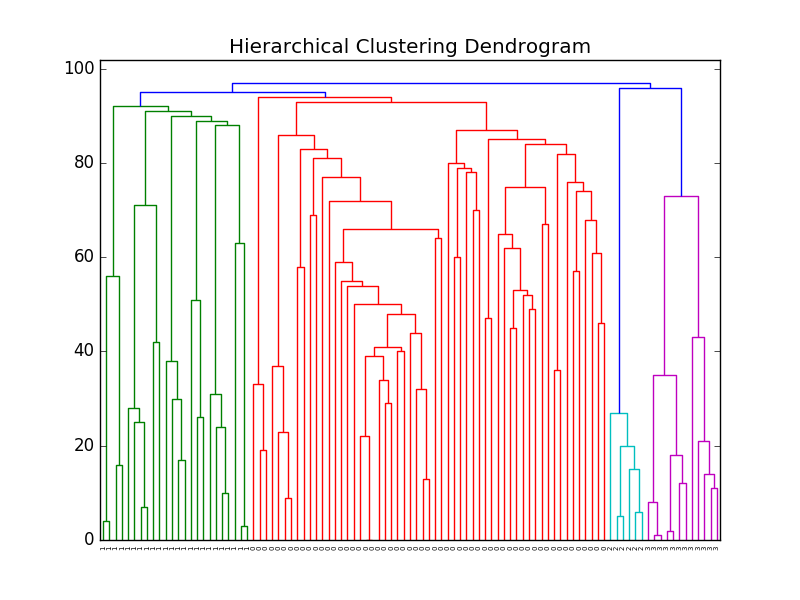
\includegraphics[width=0.75\linewidth]{pics/original_normalized.png}
  \caption{Дендрограмма кластеризуемых данных}
  \label{dendrogram_experimental}
\end{figure}

Следуя критерию большего интервала, иерархическая кластеризация формирует четыре кластера, что показано на дендрограмме \ref{dendrogram_experimental}. Визуализируя результаты спектральной кластеризации с помощью t-SNE на рисунке \ref{tsne_experimental} можно подтвердить этот вывод.
\begin{figure}[H]
	\center
  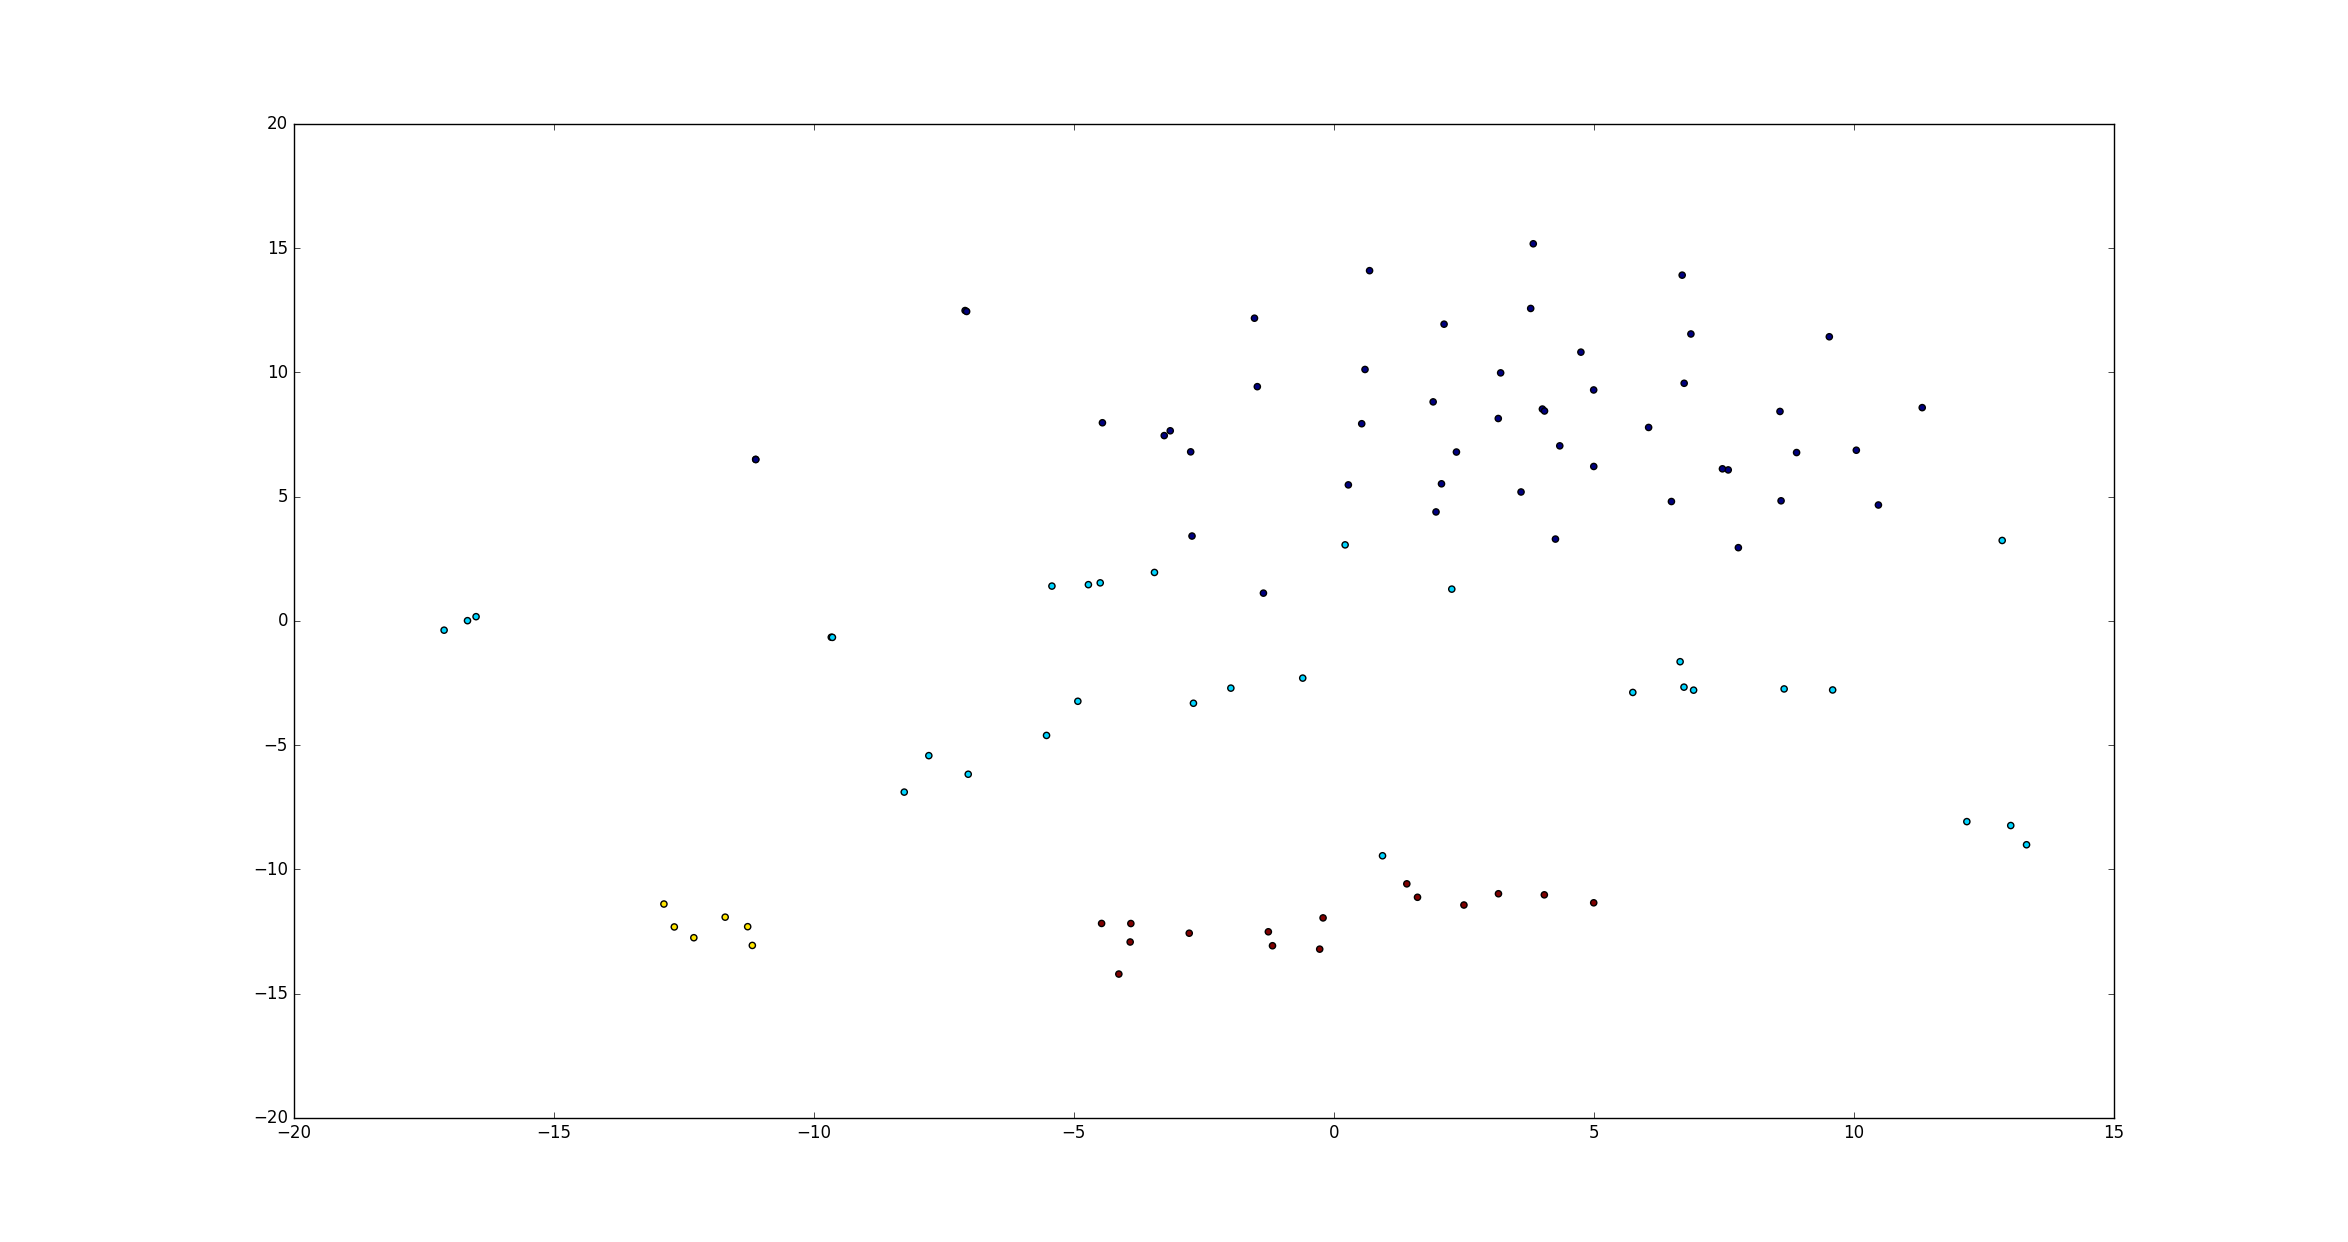
\includegraphics[width=\linewidth]{pics/tsne_color_experimental.png}
  \caption{Визуализация экспериментальных данных с помощью t-SNE}
  \label{tsne_experimental}
\end{figure}

Данное разбиение далее используется в качестве эталонного.

\subsection{Отбор признаков генетическим алгоритмом}
Генетический алгоритм, чьи параметры были определены в главе 2, был запущен на экспериментальных данных. Результатом отбора стали 35 признаков, кластеризация на которых полностью повторяет эталонную. Количество признаков, отобранное генетическим алгоритмом выбрано в качестве базового уровня для оценки ражирующих алгоритмов. 

Перечень отобранных признаков: highECI\_Motif\_1, CCC, ACGT, ACTC, AGAA, AGAC, AGAG, AGCA, AGCC, AGCG, AGCT, AGGA, AGGG, AGTG, ATCA, CACC, GGAG, TGTA, AAAAC, AAGAC, ACCGC, ACGGA, AGCTC, ATCGG, CACCA, CACTC, CCCGT, CTCAG, CTGAA, CTTGT, GCGCC, GGTCT, TACAC, TAGGC, TATAG

\subsection{Ранжирование признаков с применением спектральной теории графов}

\subsubsection{Оригинальный показатель важности}

\begin{figure}[H]
	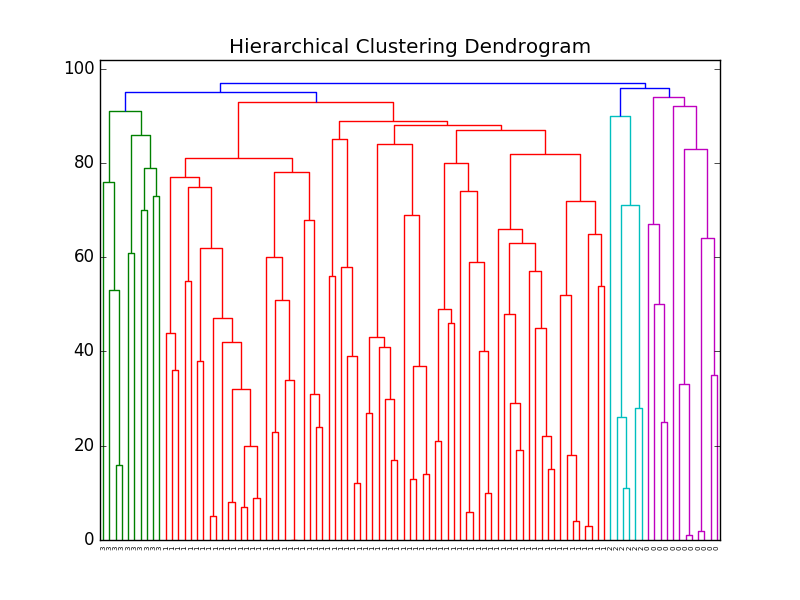
\includegraphics[width=0.5\linewidth]{pics/dendrograms/lp_norm_cosine.png}
	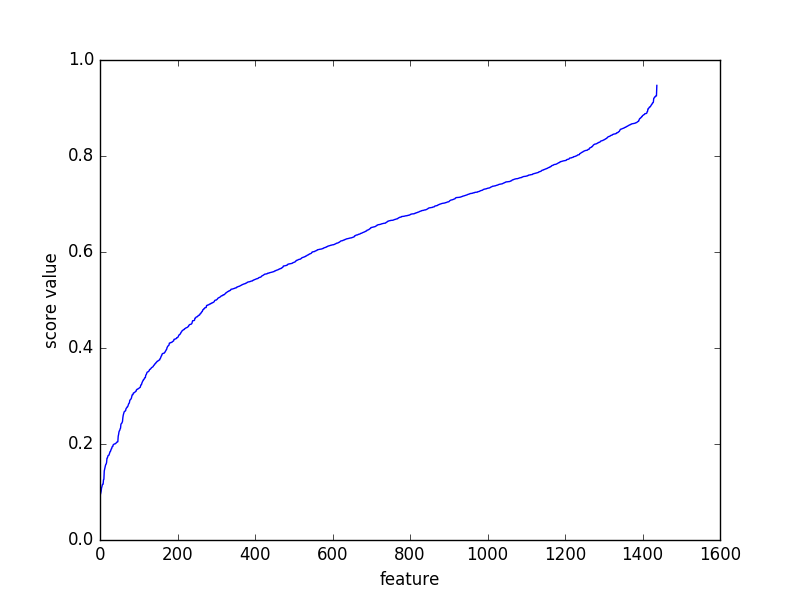
\includegraphics[width=0.5\linewidth]{pics/graphs/lp_norm_cosine.png}
	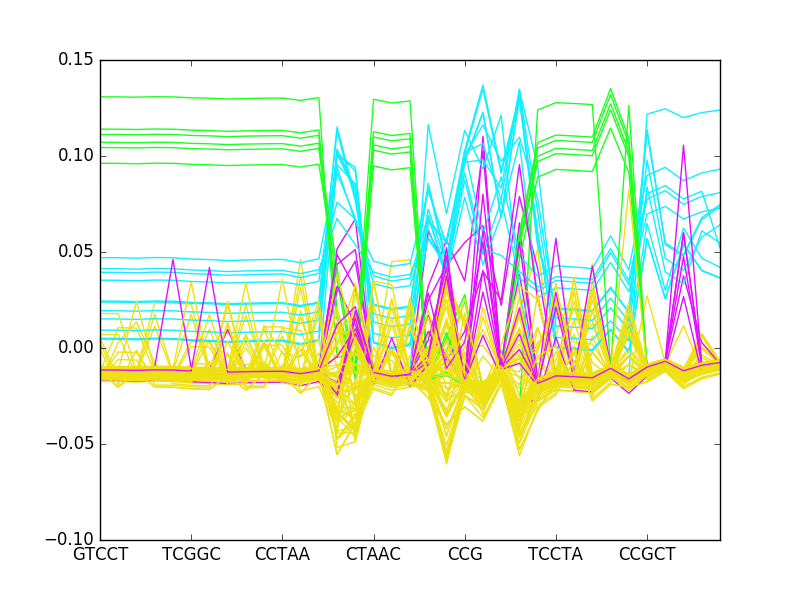
\includegraphics[width=0.5\linewidth]{pics/profiles/lp_norm_cosine.png}
	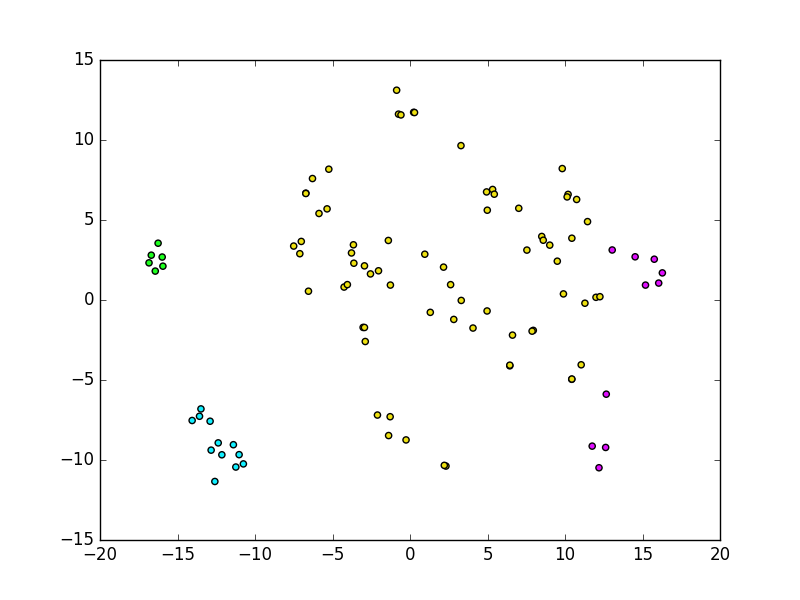
\includegraphics[width=0.5\linewidth]{pics/tsne/lp_norm_cosine.png}
	\caption{График важности признаков, дендрограмма кластеризации, t-SNE визуализация и профили экзонов на 35 наиболее важных признаках при оригинальном показателе важности на предобработанных данных}
	\label{lp_norm_cosine}
\end{figure}


\begin{figure}[H]
	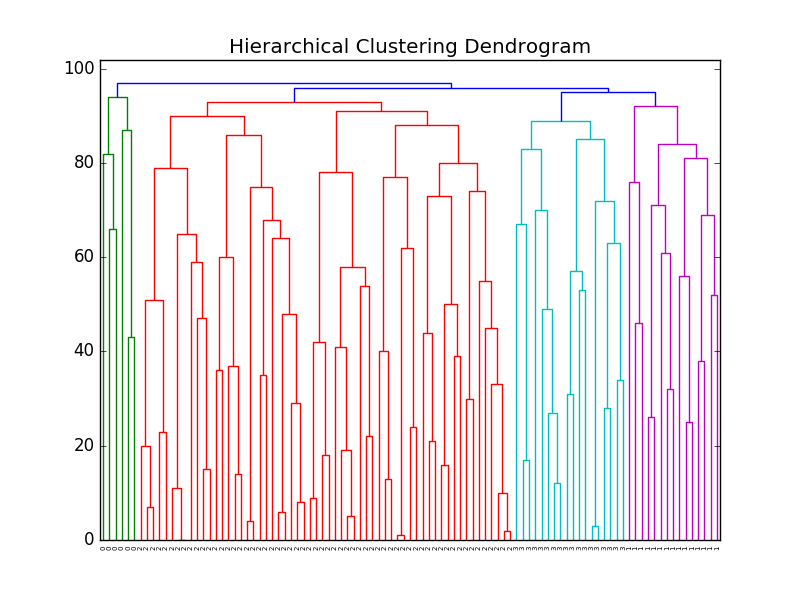
\includegraphics[width=0.5\linewidth]{pics/dendrograms/lp_unnorm_cosine.png}
	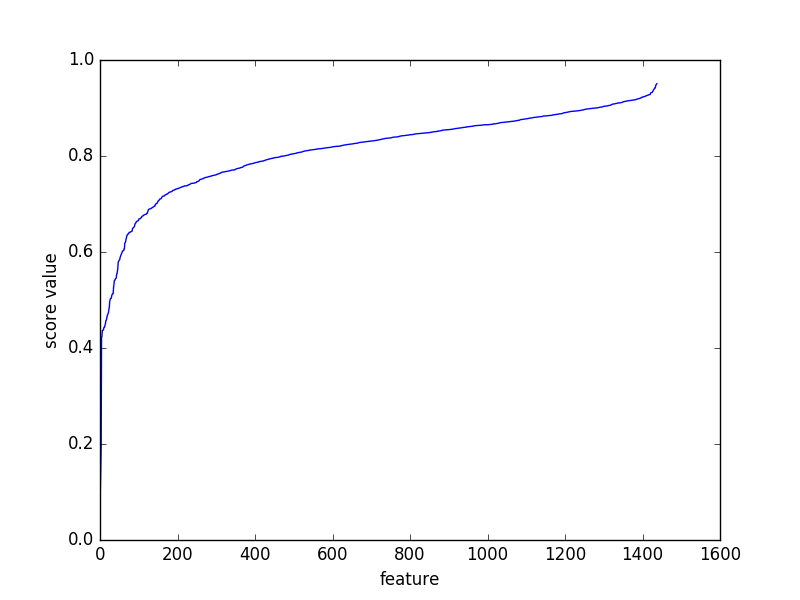
\includegraphics[width=0.5\linewidth]{pics/graphs/lp_unnorm_cosine.png}
	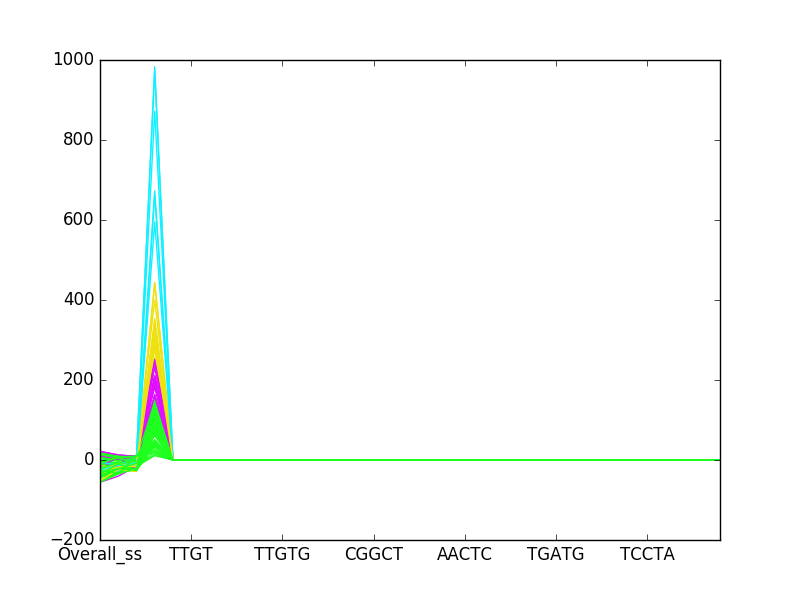
\includegraphics[width=0.5\linewidth]{pics/profiles/lp_unnorm_cosine.png}
	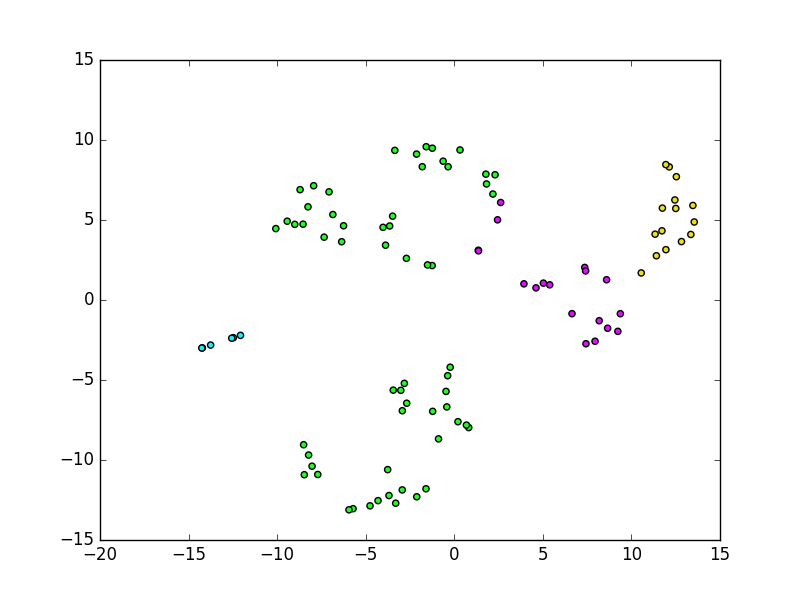
\includegraphics[width=0.5\linewidth]{pics/tsne/lp_unnorm_cosine.png}
	\caption{График важности признаков и дендрограмма кластеризации, t-SNE визуализация и профили экзонов на 35 наиболее важных признаках при оригинальном показателе важности на оригинальных данных}
	\label{lp_unnorm_cosine}
\end{figure}

\subsubsection{Использование ядер}

\begin{figure}[H]
	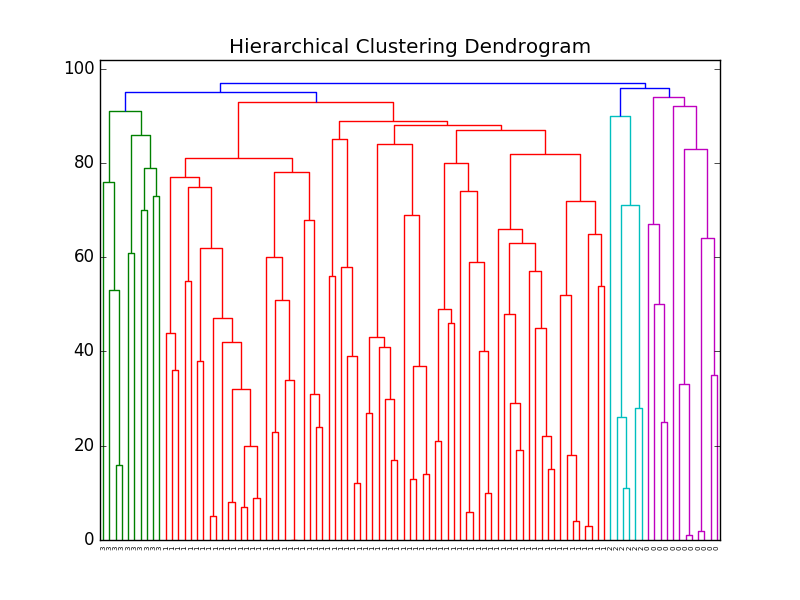
\includegraphics[width=0.5\linewidth]{pics/dendrograms/spec_norm_cosine.png}
	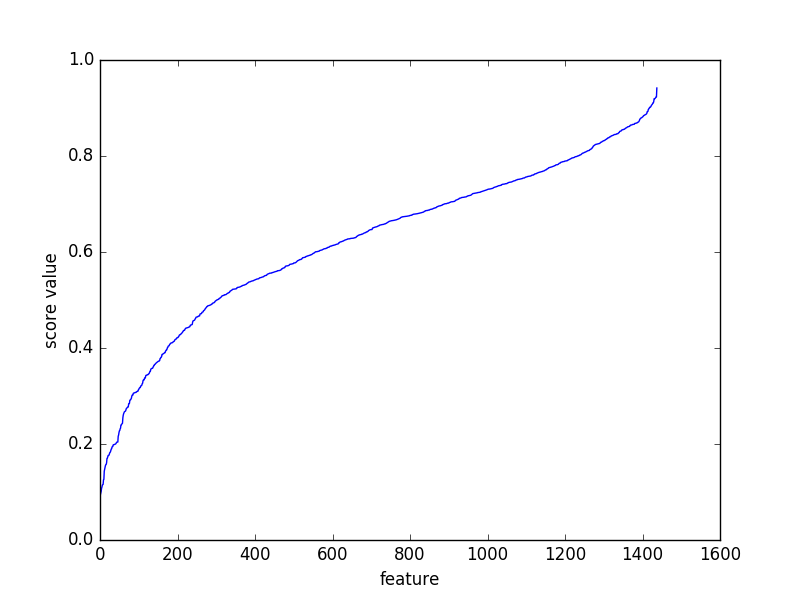
\includegraphics[width=0.5\linewidth]{pics/graphs/spec_norm_cosine.png}
	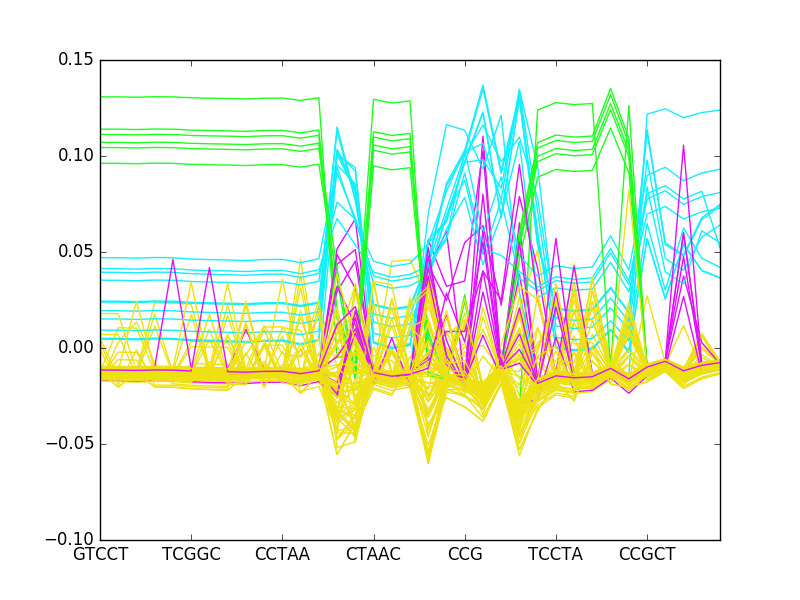
\includegraphics[width=0.5\linewidth]{pics/profiles/spec_norm_cosine.png}
	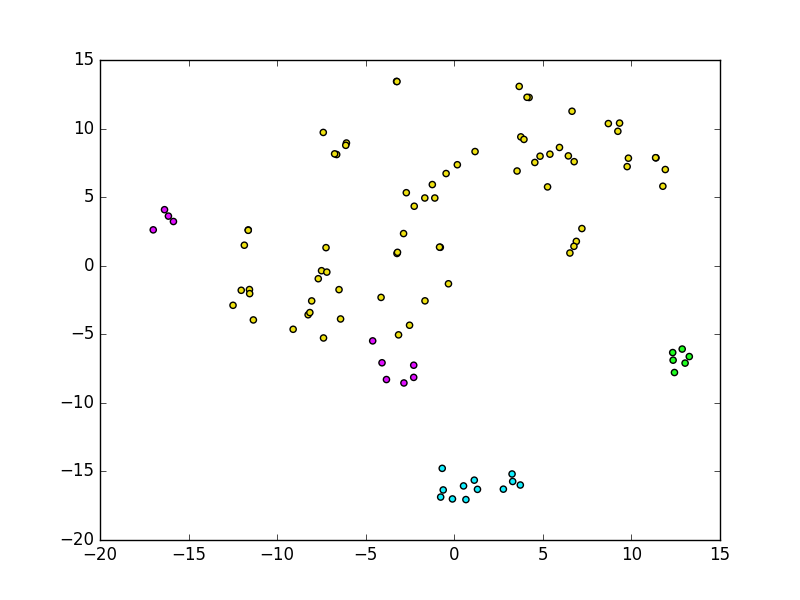
\includegraphics[width=0.5\linewidth]{pics/tsne/spec_norm_cosine.png}
	\caption{График важности признаков, дендрограмма кластеризации, t-SNE визуализация и профили экзонов на 35 наиболее важных признаках при показателе важности c ядром на предобработанных данных}
	\label{spec_norm_cosine}
\end{figure}


\begin{figure}[H]
	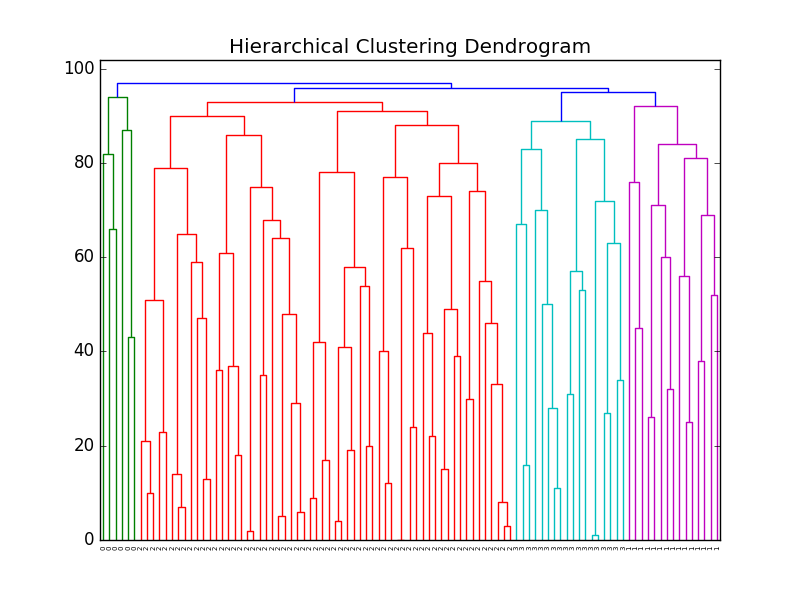
\includegraphics[width=0.5\linewidth]{pics/dendrograms/spec_unnorm_cosine.png}
	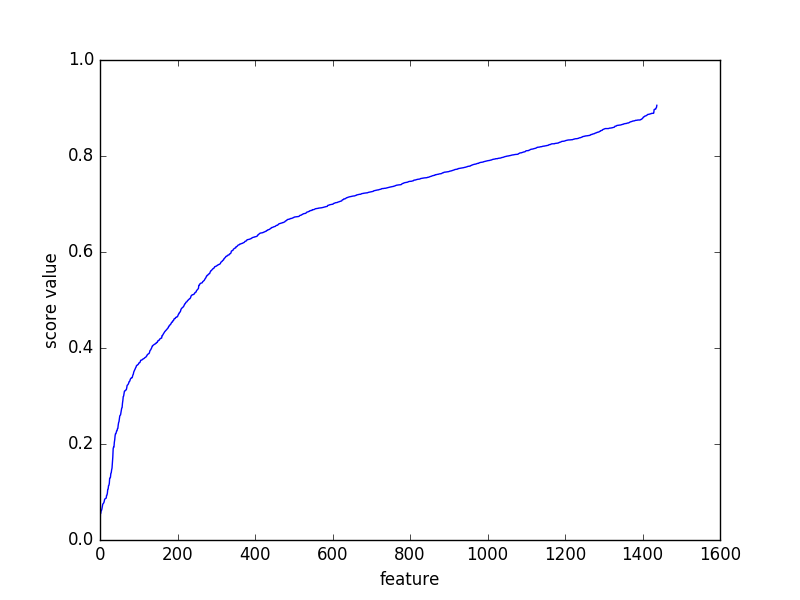
\includegraphics[width=0.5\linewidth]{pics/graphs/spec_unnorm_cosine.png}
	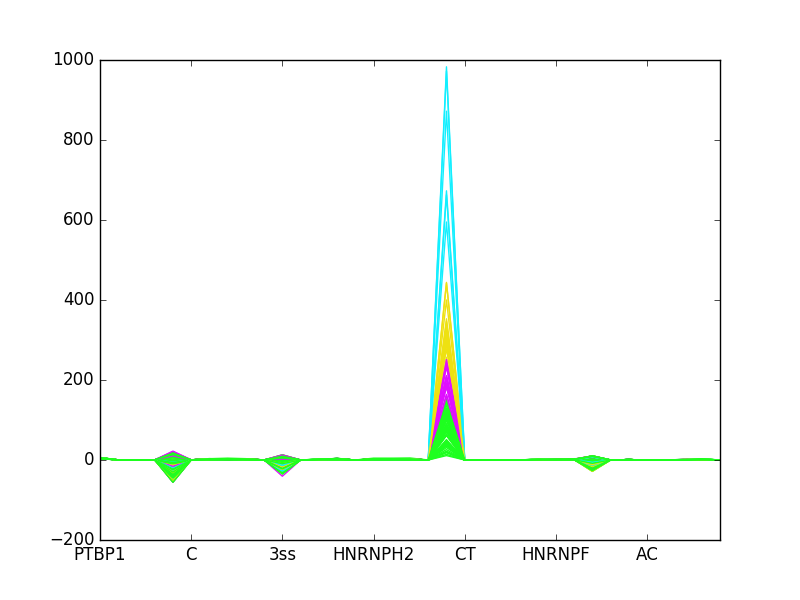
\includegraphics[width=0.5\linewidth]{pics/profiles/spec_unnorm_cosine.png}
	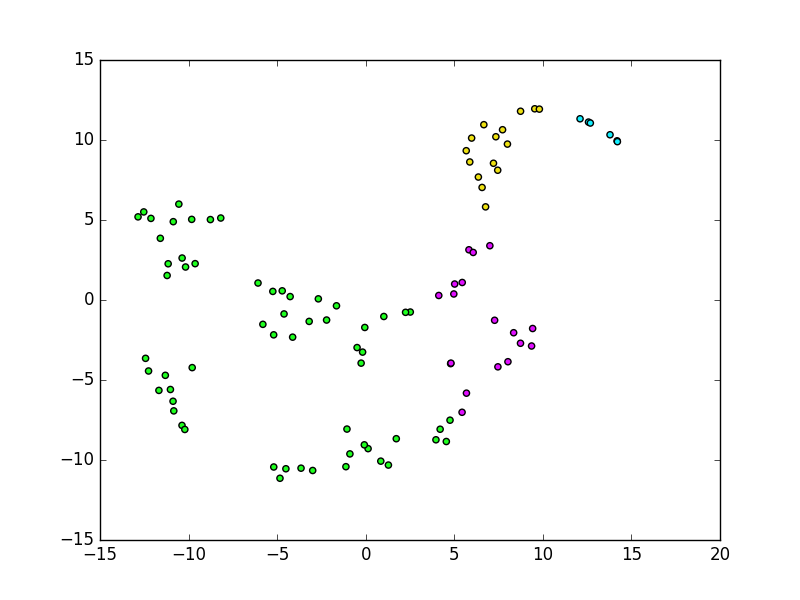
\includegraphics[width=0.5\linewidth]{pics/tsne/spec_unnorm_cosine.png}
	\caption{График важности признаков, дендрограмма кластеризации, t-SNE визуализация и профили экзонов на 35 наиболее важных признаках при показателе важности с ядром на оригинальных данных}
	\label{spec_unnorm_cosine}
\end{figure}

\subsubsection{Использование регуляризации и покластерного отбора признаков}


\begin{figure}[H]
	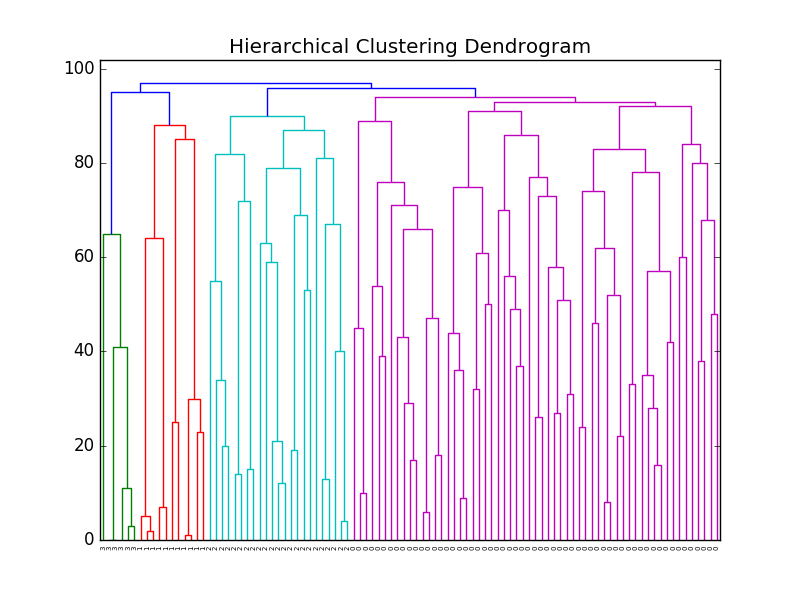
\includegraphics[width=0.5\linewidth]{pics/dendrograms/ndfs_norm_cosine_1c.png} 
	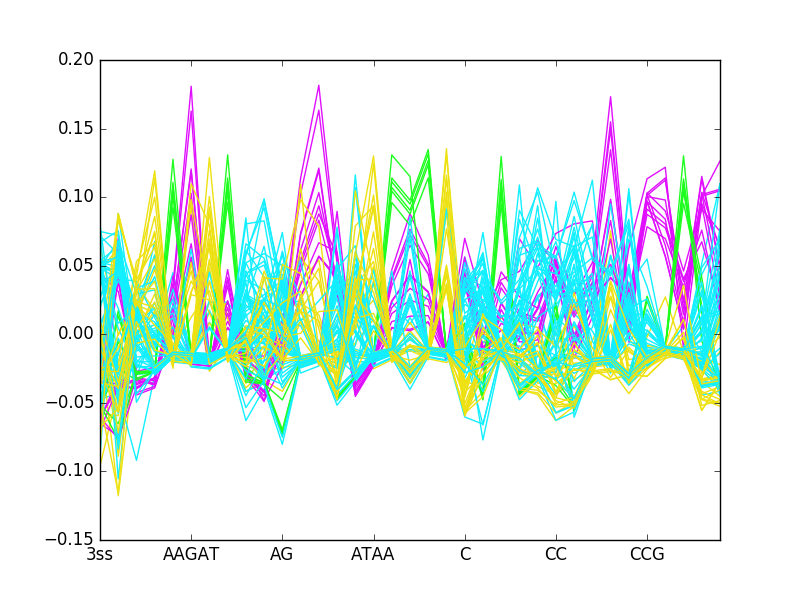
\includegraphics[width=0.5\linewidth]{pics/profiles/ndfs_norm_cosine_1c.png}
	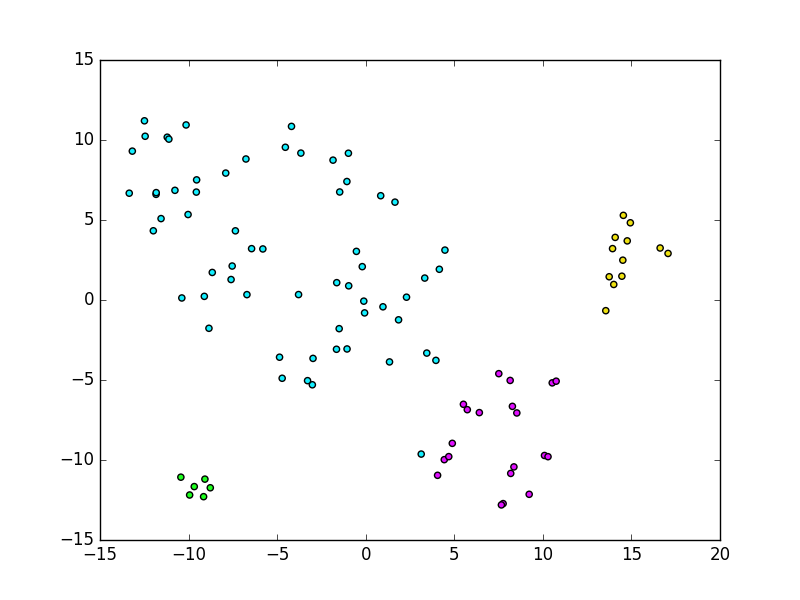
\includegraphics[width=0.5\linewidth]{pics/tsne/ndfs_norm_cosine_1c.png} \\
	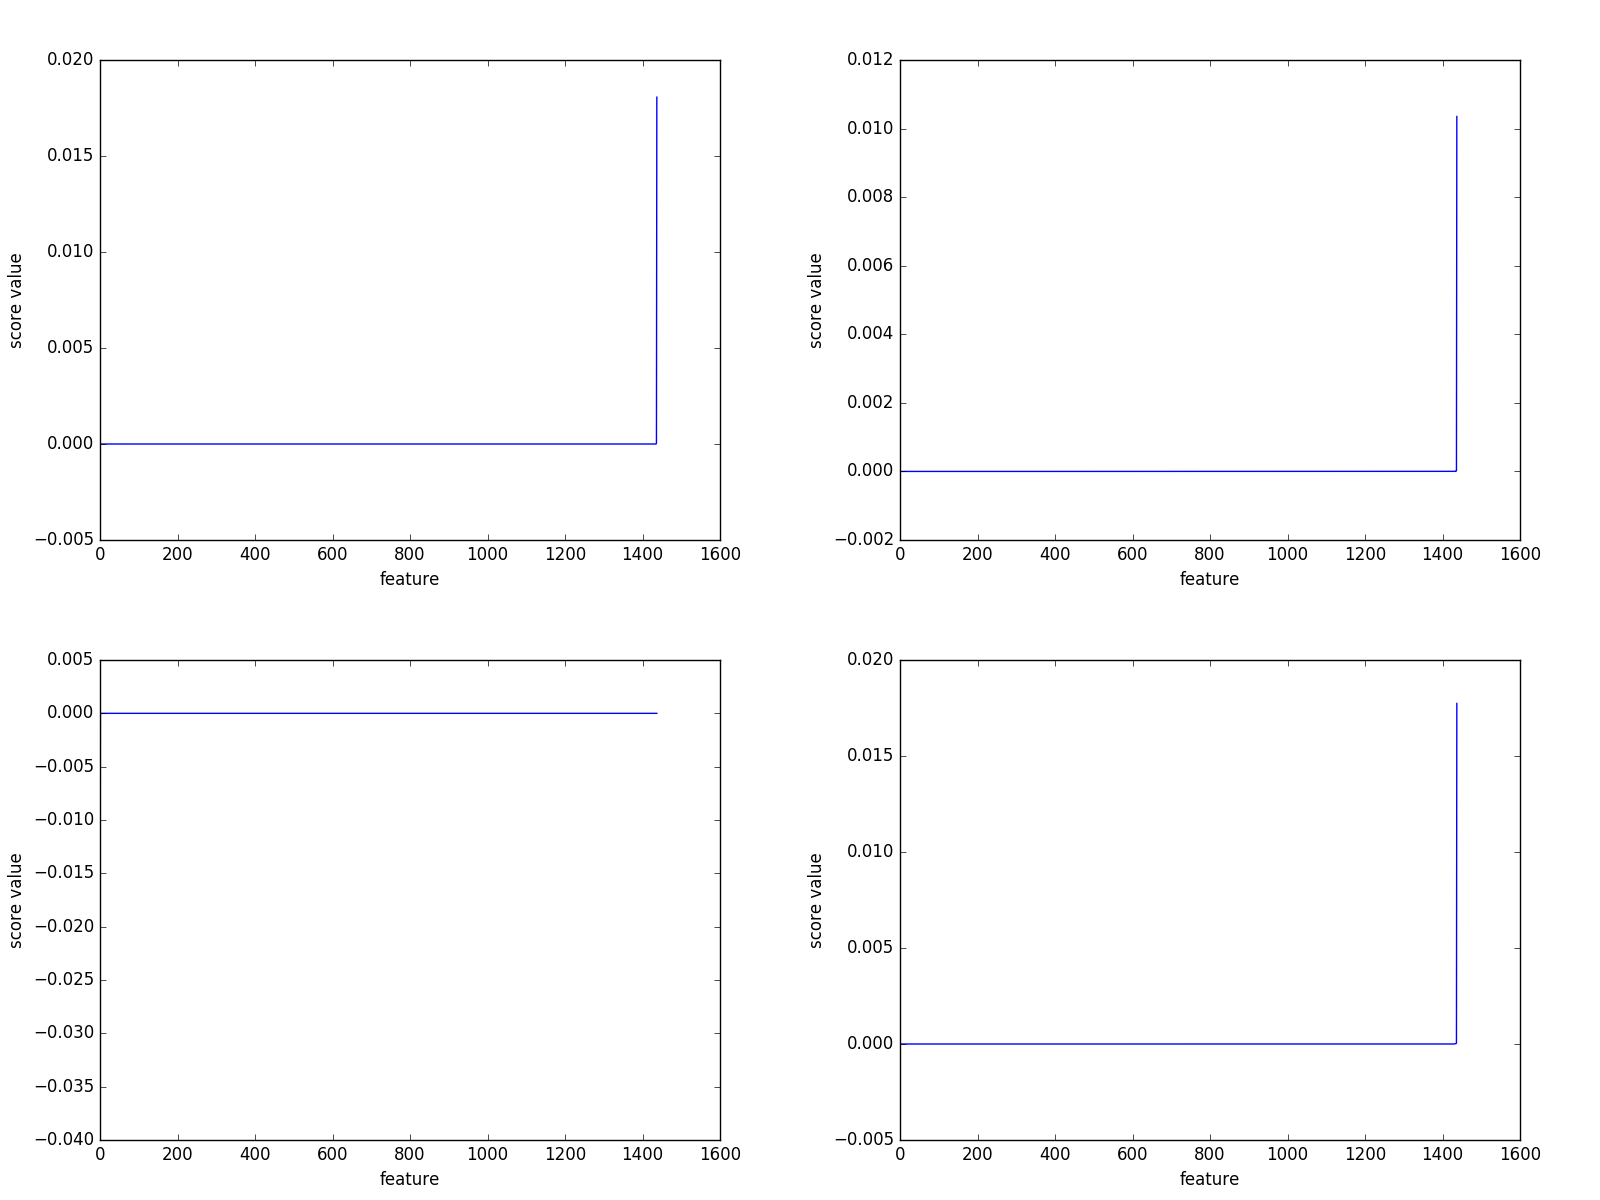
\includegraphics[width=0.8\linewidth]{pics/graphs/ndfs_norm_cosine.png}
	\caption{Покластерный график важности признаков, дендрограмма кластеризации, t-SNE визуализация и профили экзонов на 35 наиболее важных признаках при регуляризованном показателе важности на предобработанных данных}
	\label{ndfs_norm_cosine}
\end{figure}


\begin{figure}[H]
	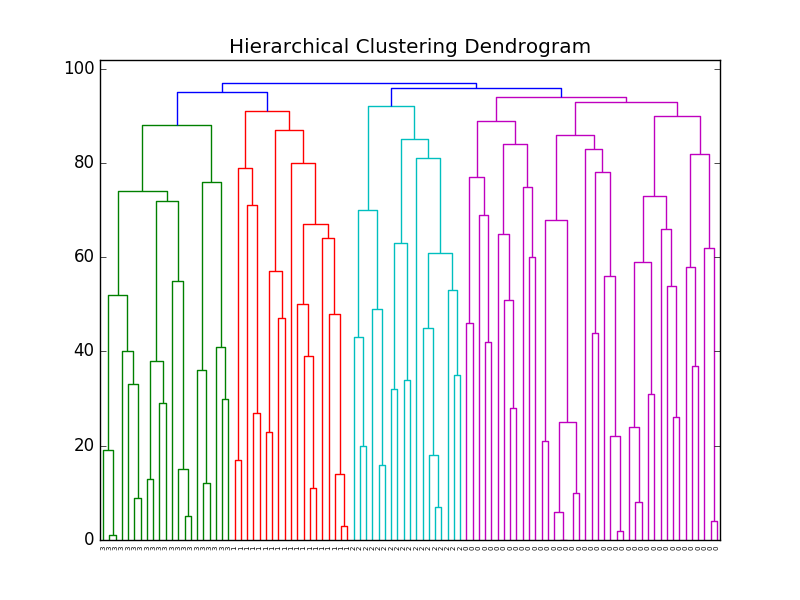
\includegraphics[width=0.5\linewidth]{pics/dendrograms/ndfs_unnorm_cosine_1c.png} 
	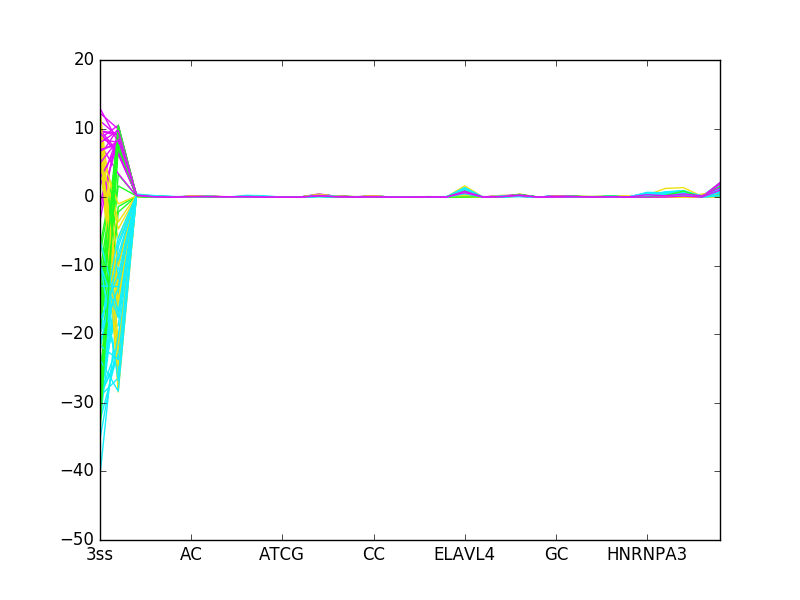
\includegraphics[width=0.5\linewidth]{pics/profiles/ndfs_unnorm_cosine_1c.png}
	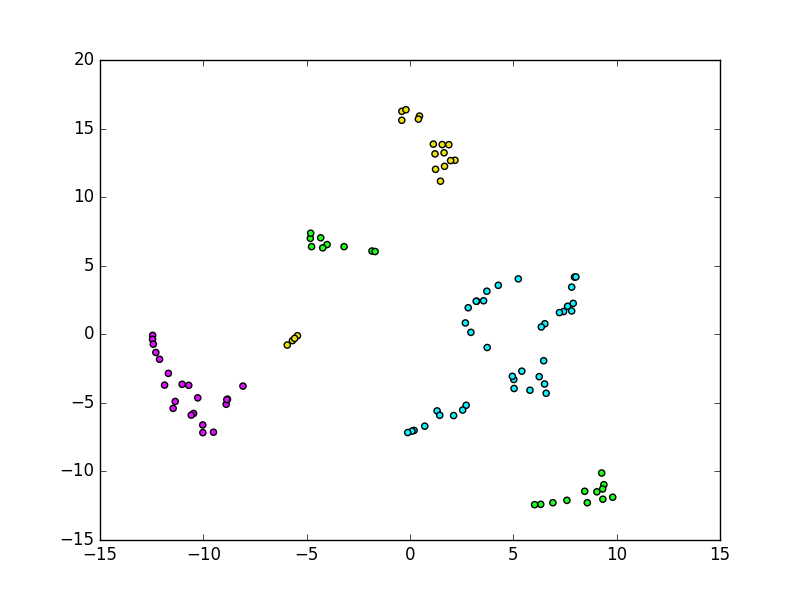
\includegraphics[width=0.5\linewidth]{pics/tsne/ndfs_unnorm_cosine_1c.png} \\
	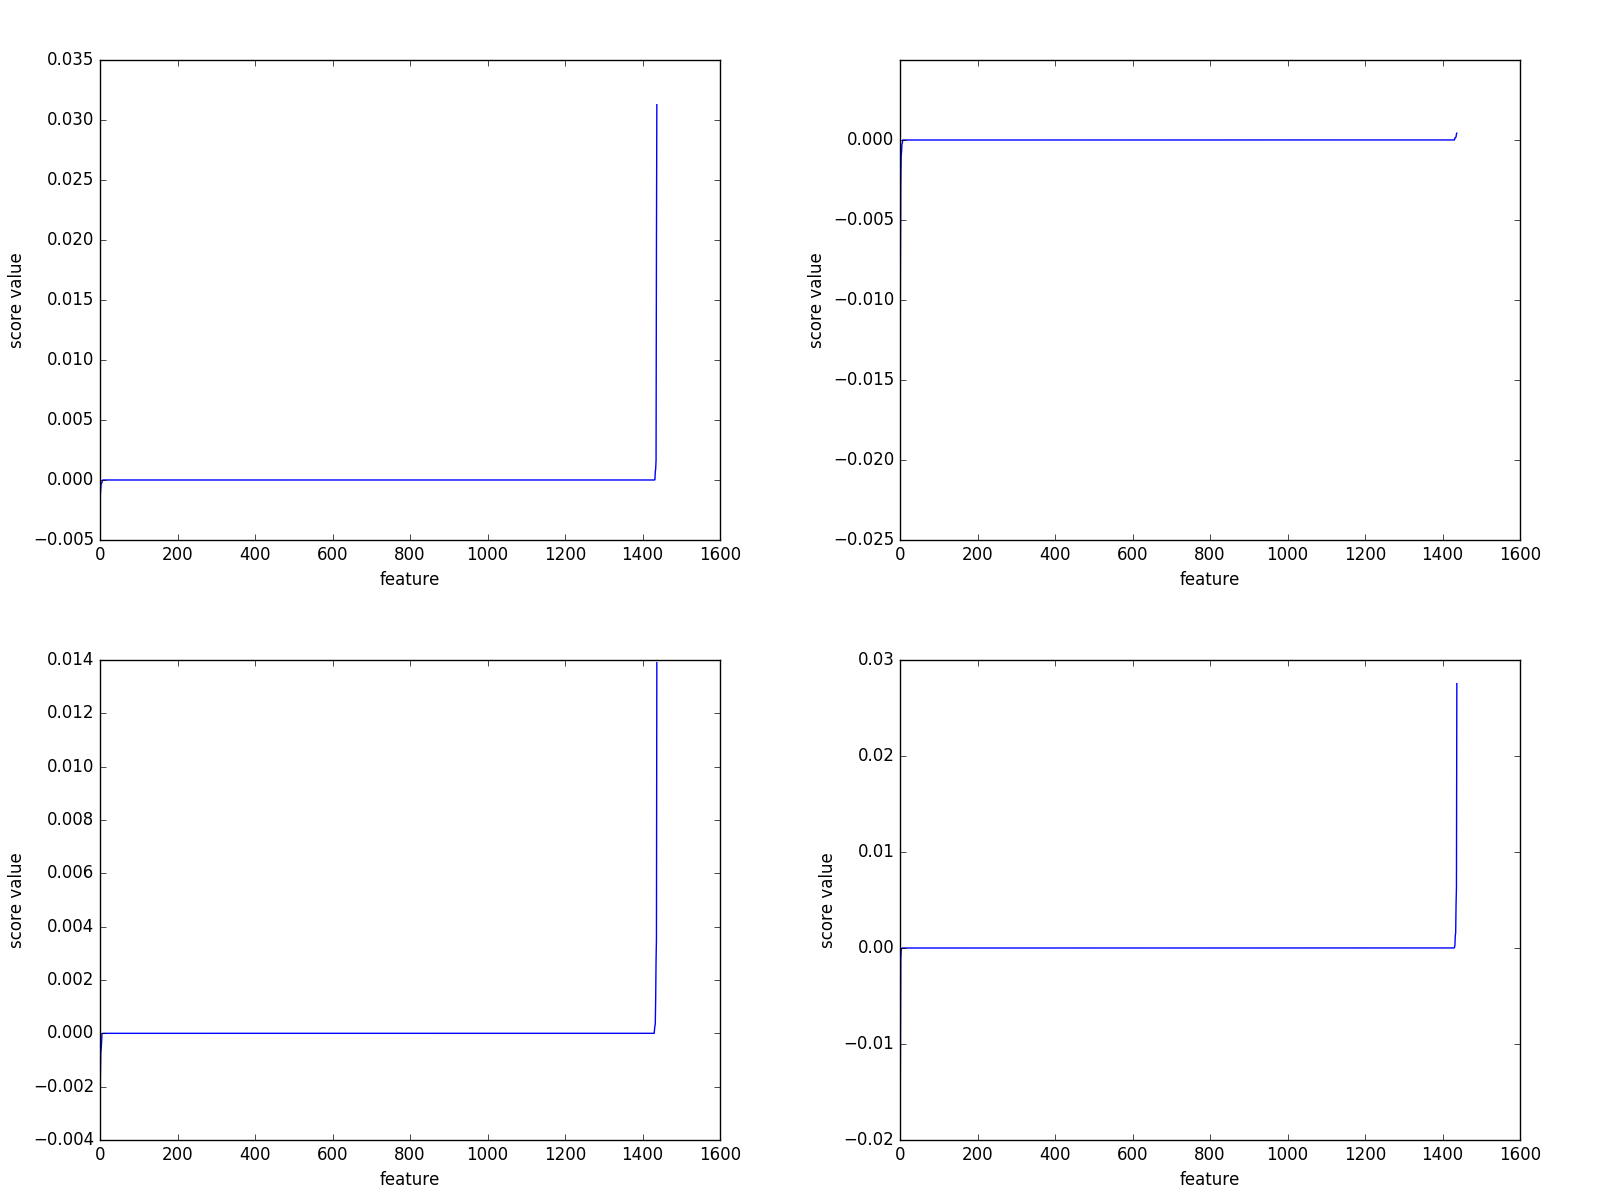
\includegraphics[width=0.8\linewidth]{pics/graphs/ndfs_unnorm_cosine.png}
	\caption{Покластерный график важности признаков, дендрограмма кластеризации, t-SNE визуализация и профили экзонов на 35 наиболее важных признаках при регуляризованном показателе важности на оригинальных данных}
	\label{ndfs_unnorm_cosine}
\end{figure}

\subsubsection{Сравнение отобранных признаков для предобработанных данных}

\begin{longtable}{|c|c|c|c|}
	\hline
	Оригинальный показатель & С ядром & Покластерный & Регуляризованный \\ \hline
	GTCCT & GTCCT & AAT & 3ss \\ \hline
GGGTC & GGGTC & AATGC & AAA \\ \hline
GGTCC & GGTCC & ACGAG & AACTC  \\ \hline
AATCG & AATCG & ACTAC & AAGAT  \\ \hline
ATCGG & ATCGG & ACTCC & AATA  \\ \hline
TCGGC & TCGGC & AGAT & AATCG  \\ \hline
GCTTG & GCTTG & AGATG & AC  \\ \hline
CAATC & CGGCT & AGGC & ACA  \\ \hline
CGGCT & CAATC & AGGCA & ACC  \\ \hline
TTGTG & TTGTG & AGTGG & ACCGC  \\ \hline
CCTAA & CCTAA & ATGTT & AGAT  \\ \hline
TGATG & TGATG & ATTCT & AGATG  \\ \hline
GTTGT & GTTGT & C & AGC  \\ \hline
CG & CG & CAATG & AGT  \\ \hline
GC & GC & CACCT & ATAA  \\ \hline
CTAAC & CTAAC & CACGA & ATCGG  \\ \hline
AACTC & AACTC & CAGAC & ATGC  \\ \hline
CTCAA & CTCAA & CGAG & ATGCG  \\ \hline
CGC & C & CGC & ATGTT  \\ \hline
C & CGC & CGGCT & ATT  \\ \hline
CCG & CCG & CTCA & C  \\ \hline
GCGC & GCGC & CTCC & CA  \\ \hline
GCCG & GCCG & CTCCA & CAATC  \\ \hline
GCG & GCG & CTTA & CAC  \\ \hline
CGGC & CGGC & GACTA & CACC  \\ \hline
TCCTA & TCCTA & GATGC & CC  \\ \hline
GGGT & TCGG & GC & CCA  \\ \hline
TCGG & GGGT & GGCAA & CCACC  \\ \hline
GCGTA & GCGTA & GGTCC & CCAGG  \\ \hline
TGTGA & TGTGA & GTAGA & CCG \\ \hline
CCGCT & CCGCT & GTCCT & CCGCT  \\ \hline
CCGCG & CCGCG & GTTGT & CCTAA  \\ \hline
CGAGC & CGAGC & MFE & CG  \\ \hline
CCGC & CCGC & SRSF9 & CGA  \\ \hline
GCCGC & GCCGC & TA & CGAG  \\ \hline
\caption{35 наиболее важных признаков для каждого подхода на предобработанных данных}
\label{features_norm}
\end{longtable}

\subsubsection{Сравнение отобранных признаков для оригинальных данных}

\begin{longtable}{|c|c|c|c|}
	\hline
	Оригинальный показатель & С ядром & Покластерный & Регуляризованный \\ \hline
Overall\_ss & PTBP1 & 3ss & 3ss \\ \hline
3ss & G & AACA & 5ss \\ \hline
5ss & T & AAGCT & A \\ \hline
Length & A & ACCGG & AA \\ \hline
AATCG & Overall\_ss & ACTC & AAA \\ \hline
TTGT & C & AGAG & AAAA \\ \hline
CCTAA & YBX1 & AGCTT & AAC \\ \hline
GTCCT & HNRNPH1 & AGG & AG \\ \hline
GTTGT & HNRNPK & AGGCA & AGG \\ \hline
GGGTC & TG & AGGG & AT \\ \hline
TTGTG & 3ss & AGGGG & ATCG \\ \hline
GGTCC & CA & ATCTT & ATGC \\ \hline
CTTGT & SFPQ & CAATG & C \\ \hline
CTCAA & PCBP1 & CAATT & CC \\ \hline
TCGGC & MFE & CCAT & CGTA \\ \hline
CGGCT & HNRNPH2 & CCCTG & CTG \\ \hline
ATCGG & HNRNPH3 & CCGGA & CTGT \\ \hline
TGTTG & MBNL1 & CCTTC & CTT \\ \hline
GCTTG & AG & CGAAA & DAZAP1 \\ \hline
CAATC & Length & CGAGT & ELAVL4 \\ \hline
AACTC & CT & CGCCT & FMR1 \\ \hline
TGT & ESEseqs & CGCGC & Fairbrother \\ \hline
TTGTT & ESSseqs & CGTC & G \\ \hline
TGTT & GA & CGTGG & GA \\ \hline
CTAAC & KHSRP & CTA & GATGC \\ \hline
TGATG & HNRNPF & CTCC & GC \\ \hline
GTGAT & PCBP2 & CTTGT & GCT \\ \hline
GATGC & 5ss & CTTTT & GCTG \\ \hline
CA & TC & GAAAG & GCTT \\ \hline
GGGT & phastCons & GACGG & GG \\ \hline
TCCTA & AC & GAG & GGC \\ \hline
TCAAT & GT & GATGC & GGT \\ \hline
GCGTA & SRSF7 & GCACA & GT \\ \hline
ATGCG & TIA1 & GCTCT & GTG \\ \hline
CGTAT & GG & GGAA & GTGG \\ \hline

\caption{35 наиболее важных признаков для каждого подхода на оригинальных данных}
\label{features_unnorm}
\end{longtable}

\subsection{Оценка отбора признаков алгоритмами из спектральной теории графов}

~

\begin{table}[H]
	\begin{tabular}{|c|c|c|}
	\hline
	Особенность алгоритма & Стандартизированные & Оригинальные \\ \hline
	Изначальный расчет показателя & 0.63 & 0.81 \\ \hline
	Применение степенного ядра & 0.66 & 0.96 \\ \hline
	Регуляризация & 0.85 & 0.07 \\ \hline
	Кластерный тбор признаков &  0.71 & 0.17 \\ \hline
	\end{tabular}
\caption{Взаимная информация для разработанного алгоритма на стандартизированных и оригинальных}
\end{table}

~

Алгоритмы отбора признаков на основе спеткральной теории графов, разработанные в главе 2, были применены к экспериментальным данным. Результаты отбора признаков представлены в таблице. Показано сохранение взаимной информации между эталонной кластеризацией и кластеризацией на 35 наиболее важных признаках. 


\newpage
\section{Основные результаты и выводы}
\begin{itemize}
	\item В главе описано применение разработанного алгоритма к экспериментальным данным
	\item Получены результаты, позволяющие сделать вывод о применимости выбранного подхода к экспериентальным данным
	\item Генетический алгоритм задает хороший базовый уровень для исследуемых алгоритмов, задав 35 признаков, полностью сохраняющих эталонное разбиение
	\item Алгоритмы на основе спектральной теории графов позволяют ранжировать признаки по важности, задавая для каждого значение показателя важности
	\item Исследовано влияние подходов различных алгоритмов к ранжированию признаков
	\item Исследуя влияние применения ядра к лапласиану графа, на рисунках \ref{spec_norm_cosine} и \ref{spec_unnorm_cosine},по сравнению с \ref{lp_unnorm_cosine} и \ref{lp_norm_cosine}, применение ядра не влияет на ранжирование при нормированных данных, но имеет влияние при оригинальных
	\item Регуляризация и внутрикластерный обтбор признаков уменьшают показатель неважных признаков, упрощая интерпретацию результата, что видно сравнивая рисунки \ref{ndfs_unnorm_cosine} и \ref{ndfs_norm_cosine} с \ref{lp_unnorm_cosine} и \ref{lp_norm_cosine}
	\item Для каждого подхода отобраны 35 наиболее важных признаков, что позволяет сравнить результаты работы алгоритмов с отобранными генетическим алгоритмом. Анализ таблиц \ref{features_norm} и \ref{features_unnorm} показывает, что в случае оригинальных данных большое влияние показывают признаки с высокой дисперсией, что подтверждает гипотезу, высказанную в начале главы. Множества признаков, отобранные на предобработанных данных схожи между собой и множеством признаков, отобранным генетическим алгоритмом, что позволяет выделить эти признаки как наиболее важные. 
\end{itemize}


%%% описание заключения

\settocdepth{chapter}

\setcounter{chapter}{0}
\phantomsection
\chapter*{ЗАКЛЮЧЕНИЕ}
\addcontentsline{toc}{chapter}{Заключение}

\begin{itemize}
	\item Были рассмотрены актуальные подходы в выделении важных признаков в задаче кластеризации. В качестве основного выбран подход, основанный на спектральной теории графов.
	\item Выбрана модель CRISP-DM для решения поставленной задачи отбора экзонных признаков. Модель характиризуется широкой применимостью и иерархической структурой, позволяющей делить задачи.
	\item Построена модель для генерации кластеризированных данных для разработки алгоритма. Модель генерирует многомерные нормальные кластеры с возможностью задания связей между компонентами.
	\item Были описаны и проанализированы алгоритмы кластеризации и визуализации многомерных данных. В качестве кластеризации ыбл выбран алгоритмы иерархической и спектральной кластеризации, хорошо подходящие для поиска структуры в данных, а в качестве визуализации был выбран алгоритм t-SNE, пригодный для построения низкоразмерного отображения исходных данных.
	\item Построен алгоритм для оценивания результатов кластеризации с помощью теоретико-информационных подходов
	\item Построен алгоритм отбора признаков, включающий различные подходы и оценку результата, в том числе комбинаторную оптимизацию
	\item Обоснован выбор технических средств для реализации алгоритма
	\item В экспериментальных данных выделены наиболее важные признаки, задающие кластерную структуру.
	\item Установлен факт ненормальности экзонных признаков и влияние факта на процесс отбора признаков
	\item Подготовлены направления для дальнейшего развития исследования
	\item Работа выполнена при участии в НИР 834/18
	\item Результаты исследования по кластеризации экзонов онкогена доложены на международной конференции CSIST'2016, статья опубликована в сборнике трудов конференции
\end{itemize}

%%% описание библиографии

\nocite{*}
\cleardoublepage
\phantomsection
\addcontentsline{toc}{chapter}{Список использованной литературы}

{\small \bibliography{diploma-bibliography}}

\phantomsection
% хак для выравнивания слова "Приложение" по правому краю - куча неразрывных пробелов:
\chapter*{~~~~~~~~~~~~~~~~~~~~~~~~~~~
  ~~~~~~~~~~~~~~~~~~~~~~~~~~~
  ПРИЛОЖЕНИЕ А\\
  ИСХОДНЫЙ КОД}
\addcontentsline{toc}{chapter}{Приложение А. Исходный код}
\stepcounter{attachcnt}

Lorem ipsum dolor sit amet, consectetur adipiscing elit. Fusce ultrices finibus arcu in tincidunt.
Curabitur pellentesque purus vel aliquet efficitur. Morbi quis placerat diam. Curabitur id fringilla
nibh, eu volutpat tellus. Sed nec fermentum magna, eget blandit ipsum. Aenean fermentum ipsum eu
luctus vulputate. In hendrerit eros nibh, non pretium eros malesuada nec. Donec enim lectus, convallis
id scelerisque a, molestie nec neque.

Integer fermentum, dui volutpat suscipit scelerisque, orci sapien suscipit mauris, nec bibendum est
enim elementum sem. Mauris pharetra turpis eget ex tincidunt, in efficitur mi dictum. Suspendisse
convallis non lacus nec fermentum. Suspendisse eleifend enim odio, sed eleifend felis luctus eget.
In bibendum nulla a lorem tempor dignissim. Nunc tempor arcu a nisl feugiat, a fermentum ante eleifend.
Etiam sed augue lacinia, luctus odio sed, dapibus lacus. Pellentesque suscipit mauris vitae est
fringilla consequat. Sed dui est, varius sit amet auctor ut, euismod a magna. Vivamus tristique leo
ligula, non lacinia justo volutpat in. Maecenas eu mi velit. Sed vel elit ligula. In imperdiet varius
elit, at rutrum mauris lobortis nec. Suspendisse quis orci id urna porta eleifend.

Curabitur pellentesque nunc ut urna elementum bibendum. Maecenas sit amet ante tincidunt, dictum
neque et, eleifend felis. Pellentesque rhoncus mi ut mauris ullamcorper pretium. Maecenas non blandit
ex, quis elementum leo. Donec ultricies, velit in ultricies fringilla, turpis neque facilisis eros,
non congue ipsum sapien id enim. Praesent vitae tellus ornare orci mattis ornare et ut sapien. Quisque
iaculis lorem mauris. Phasellus eu arcu placerat, convallis velit at, tincidunt velit. Nulla eget
vestibulum erat. Fusce eu ipsum rutrum, varius felis dictum, aliquam augue.

In dignissim odio eget porttitor malesuada. Pellentesque venenatis urna eget risus facilisis
imperdiet. Donec ligula neque, volutpat ut leo in, interdum pellentesque metus. Nam mattis ligula
nec volutpat fringilla. Pellentesque nec semper mauris, non condimentum metus. Ut imperdiet sapien
nec pretium porta. Nam id arcu non nibh ultricies consectetur id sed dui.

Duis semper luctus posuere. Donec aliquet quam a ex posuere venenatis. Aliquam interdum suscipit
justo, placerat auctor lacus feugiat eget. Aliquam vulputate vitae lorem at molestie. In iaculis
felis in felis rutrum, eget finibus nunc gravida. Curabitur tortor tortor, rutrum eu urna ut, commodo
tempor justo. Quisque at tortor nec leo fringilla posuere.

Fusce sapien nisl, gravida et eleifend vitae, finibus at quam. Curabitur quis venenatis nisl.
Aenean in rhoncus magna. In hac habitasse platea dictumst. Nulla id feugiat nibh. Suspendisse ut
ligula at elit auctor aliquet. Quisque dolor nunc, pretium vitae posuere dapibus, molestie ac lectus.
Nulla tempor dui lacinia auctor finibus. Curabitur placerat diam non augue posuere accumsan. Nunc
laoreet urna mi, eget faucibus ligula faucibus at. Nunc eu laoreet erat. Suspendisse varius est orci,
ut scelerisque metus faucibus non. Donec luctus et massa non semper. Nullam non augue enim. Aliquam
vitae convallis ligula. Interdum et malesuada fames ac ante ipsum primis in faucibus.

\begin{figure}
  
\includegraphics[width=\linewidth]{pics/hardcore.jpg}
  \caption{Учеба - это хардкор. Диплом - это дважды хардкор.}
  %\label{fig:hard}
\end{figure}



\end{document}
